\documentclass[11pt, a4paper]{article}

%\usepackage[german]{babel}
\usepackage[english]{babel}
\usepackage{BT_titlepage}

\RequirePackage[utf8]{inputenc}
\RequirePackage[T1]{fontenc}
\RequirePackage[pdftex,paper=a4paper,margin=3cm]{geometry}
\RequirePackage[pdftex]{graphicx}
\RequirePackage[unicode=true, hidelinks]{hyperref}
\RequirePackage{subcaption}
\RequirePackage[usenames, dvipsnames]{color}
\RequirePackage{mathptmx}
\RequirePackage{setspace}
\RequirePackage{lineno}
\RequirePackage{threeparttable}
\RequirePackage{array}
\RequirePackage{booktabs}
\RequirePackage{appendix}
\RequirePackage{multirow}
\RequirePackage{amsmath}
\RequirePackage{amsfonts}
\RequirePackage{amssymb}
\RequirePackage{nameref}
\RequirePackage{placeins}
\RequirePackage{gensymb}
\RequirePackage{listings}
\RequirePackage{cleveref}
\RequirePackage{mathrsfs}
\RequirePackage{authblk}

%\linenumbers
\onehalfspacing

% code listing formatting
%\definecolor{codegreen}{rgb}{0,0.6,0}
%\definecolor{codegray}{rgb}{0.5,0.5,0.5}
%\definecolor{codepurple}{rgb}{0.58,0,0.82}
%\definecolor{codered}{RGB}{160,0,0}
%
%\definecolor{backcolour}{rgb}{0.95,0.95,0.92}
%\definecolor{backcolour-arian}{RGB}{253,246,227}
%\definecolor{keywords}{RGB}{203,75,22}
%\definecolor{comments}{RGB}{42,161,152}
%
%\lstset{
%	language=Python,
%    backgroundcolor=\color{backcolour},   
%    commentstyle=\color{codegreen},
%    %keywordstyle=\color{codepurple},
%    stringstyle=\color{codered},
%	basicstyle=\ttfamily,
%	columns=fixed,
%	%frame=single,
%    breaklines=true,
%    breakatwhitespace=true,
%    postbreak=\mbox{\textcolor{red}{$\hookrightarrow$}\space},
%    keepspaces=true,
%    showstringspaces=false,
%%    aboveskip=-1.3em,
%%    belowskip=0.3em,
%%    upquote=true,
%}

% arian
% configure listings to highlight Python code
%\definecolor{keywords}{RGB}{203,75,22}
%\definecolor{comments}{RGB}{42,161,152}
%\definecolor{red}{RGB}{160,0,0}
%\definecolor{green}{RGB}{0,150,0}
%\definecolor{bg}{RGB}{253,246,227}
% 
% \lstset{language=Python, 
%         basicstyle=\ttfamily\small, 
%         keywordstyle=\color{keywords},
%         commentstyle=\color{comments},
%         %stringstyle=\color{red},
%         showstringspaces=false,
%         %identifierstyle=\color{green},
%         procnamekeys={def,class},
%         backgroundcolor=\color{bg},
%         }

\newcommand{\giturl}{\url{github.com/ariansajina/bachelor-thesis}}

\usepackage{accents}
\newcommand{\ubar}[1]{\underaccent{\bar}{#1}}

\usepackage{amsthm}
\theoremstyle{definition}
\newtheorem{assumption}{Assumption}
\newtheorem{definition}{Definition}

% Configure references
\RequirePackage[backend=biber, citestyle=authoryear, style=authoryear, sorting=none, natbib=true, maxnames=3, minnames=1, maxcitenames=1, mincitenames=1, url=false, giveninits=true, sortcites=true, date=year, doi=false,isbn=false]{biblatex}

\renewbibmacro*{volume+number+eid}{%
  \printfield{volume}%
  \setunit*{\addnbthinspace}
  \printfield{number}%
  \setunit{\addcomma\space}%
  \printfield{eid}}
\DeclareFieldFormat[article]{number}{\mkbibparens{#1}}
\renewbibmacro*{in:}{}
\DeclareFieldFormat
  [article,inbook,incollection,inproceedings,patent,thesis,unpublished]
  {title}{#1\isdot}
\DeclareFieldFormat{pages}{#1}
\renewcommand*{\bibpagespunct}{\addcolon\space}

\renewcommand{\thesubfigure}{\Alph{subfigure}} % Uppercase subfigure letters
\renewcommand{\floatpagefraction}{.85}%
\renewcommand{\topfraction}{.85}%
\renewcommand{\bottomfraction}{.50}%

\newcommand\numberthis{\addtocounter{equation}{1}\tag{theequation}}

% indicator function
\RequirePackage{bbm}
%\RequirePackage{anyfontsize}
%\def\one{\mbox{1\hspace{-4.25pt}\fontsize{12}{14.4}\selectfont\textrm{1}}}

%Namen des Verfassers der Arbeit
\author{Arian \v{S}ajina}
%Geburtsdatum des Verfassers
\geburtsdatum{June 8, 1996}
%Gebortsort des Verfassers
\geburtsort{Pula, Croatia}
%Datum der Abgabe der Arbeit
\date{\today}

%Name des Betreuers
% z.B.: Prof. Dr. Peter Koepke
\betreuer{Supervisor: Prof. Dr. Anton Bovier}
%Name des Zweitgutachters
\zweitgutachter{Second assessor: Prof. Dr. Patrik Ferrari}
%Name des Instituts an dem der Betreuer der Arbeit tätig ist.
%z.B.: Mathematisches Institut
%\institut{Mathematisches Institut}
\institut{Institut f\"ur Angewandte Mathematik}
%\institut{Institut f\"ur Numerische Simulation}
%\institut{Forschungsinstitut f\"ur Diskrete Mathematik}
%Titel der Bachelorarbeit
\title{Adaptive Dynamics and the Evolution of Ageing}
%Do not change!
\ausarbeitungstyp{Bachelor's thesis mathematics}

\bibliography{references}

\begin{document}

\maketitle

\clearpage

\tableofcontents
\newpage

\section*{Zusammenfassung}
    Evolution des Alterns in biologischen Systemen ist immer noch ein ungel\"ostes Problem. Diese Arbeit motiviert wie, im Fall einer klonalreproduzierenden Population, individuellbasierte stochastische Modelle mit etablierten evolution\"aren Theorien des Alterns kombiniert sein k\"onnen.
    Es wird das individuellbasierte Modell der Theorie der adaptiven Dynamik eingef\"uhrt, und sowohl eine spezielle Wahl der Parametrisation der Geburten- und Sterberate, als auch verschiedene Weisen auf die Mutation die Merkmale beeinflussen kann diskutiert.
    Die Parametrisation suggeriert, dass die Geburten- und Sterberate als Treppenfunktionen des Alters zu betrachten und die Merkmale alterspezifisch sind.
    Schlie\ss{}lich wird das stochastische Modell in Python implementiert und einige Ergebnisse aus numerischen Simulationonen werden vorgef\"uhrt. Die Ergebnisse zeigen, dass mit dieser Parametrisation alternde Phenotype als Folge der evolution\"aren Prozesse zu Stande kommen k\"onnen.

\section*{Abstract}
    Evolution of ageing in biological systems is still an unresolved problem. This thesis motivates how, in the case of clonally reproducing populations, individual-based stochastic models can be combined with established evolutionary theories of ageing. 
    The individual-based model of adaptive dynamics with age structure is introduced and a special choice of parametrization for the birth and death rate is discussed, as well as different possible ways in which mutation can act on the traits. 
    The parametrization suggests to consider birth and death rate as step-functions of age, and traits to be age-specific.
    Finally, the stochastic model is implemented in Pyhton and results from numerical simulation are presented, which show that with the above parametrization, ageing phenotypes can evolve in this model.

%\large\textbf{Keywords:} evolution of ageing, adaptive dynamics, life-history, numerical simulations

\section{Introduction}
    What is ageing and why do organisms age? Although all of us possess some intuition about these questions, exact answers continue to elude us. Broadly, biological ageing or \emph{senescence} is characterized as the decline in performance of biological systems with age. In evolutionary biology, senescence is defined as an age-dependent increase in mortality and decline in fecundity \autocite{rose1991}.
    
    It has long been dismissed that ageing is just an inevitable result of the damage an organism accumulates over its lifetime, since some organisms demonstrate the capability of repair and maintenance; most notably the Hydra do not appear to age at all. On the other hand, the phenomenon of ageing is widely spread in the animal kingdom and we observe that the age-dependent rates of mortality and fecundity vastly differ in nature both across and within taxa \autocite{jones2014diversity}. For
    instance some oaks are known to live for well over 150 years, while some mayflies live only a couple of hours in their adult form. Moreover, the domesticated brown rat lives for 2-3 years, while the naked mole rat, besides being an extraordinarily interesting mammal, can live for more than 30 years \autocite{naked-mole-rat}.
%TODO maybe add citation of work where genetic intervention has prolonged lifespan, either here or in discussion later?

    These striking differences strongly indicate that ageing is to a nontrivial extent shaped by evolutionary processes. Although this might at first seem paradoxical, since natural selection should supposedly maximize fitness, i.e.\ survival and reproductive capacity, a succession of authors has provided us with a theoretical framework for investigating the evolution of ageing. 
    This framework naturally comes to consider a population with an age structure, for the ageing part, and some hereditary element, for the evolution part.
    Although not aimed at investigating the evolution of ageing from the outset, extensive mathematical theory has been developed to describe these two phenomena; namely the behaviour of age-structured populations and the change of genotype frequencies over time, with focus on long-term behaviour under a large population limit.

    The remainder of this section provides the reader with a brief overview of the key ideas from evolutionary biology that first raised the question of evolution of ageing, as well as of mathematical models and computer simulations that can be or were utilized to study this problem. With mathematical models the focus is kept on works that play into the model that will ultimately be considered in later sections of this thesis.
    %Similarly, with computer simulations, only works that directly address evolution of ageing are mentioned.
    
\subsection{Population dynamics}
    Population growth as a subject of study first gained prominence with the work of Malthus, who proposed a model in which population growth is proportional to population size \autocite{malthus1798}. In this model the population size $P(t)$ at time $t\geq 0$ satisfies the differential equation:
    \begin{equation}
        \frac{d}{dt} P(t) = r P(t).
    \end{equation}
    The solution is given by $P(t) = e^{rt}P(0)$ and here $r\in \mathbb{R}$ is called the malthusian parameter and describes the growth rate of the population. The model suggests that for $r>0$, the population would grow indefinitely; an unrealistic property.
    This was addressed by Verhulst, resulting in his famous \emph{logistic equation} in which the malthusian parameter depends on population size itself and growth abates as population size approaches the limit that its environment can sustain \autocite{verhulst1838}. In this model the population function $P(t)$ satisfies the differential equation:
    \begin{equation}\label{eq:verhulst}
        \frac{d}{dt} P(t) = r \Big(1 - \frac{P(t)}{K} \Big) P(t).
    \end{equation}
    Here $r\geq 0$ is called the \emph{intrinsic growth rate} and $K>0$ is called the \emph{carrying capacity}. Equation \eqref{eq:verhulst} can be solved by separation of variables to yield
    \begin{equation}\label{eq:verhulst2}
        P(t) = \frac{K}{1+(K/P(0)-1)e^{-rt}}
    \end{equation}
    It is clear from equation \eqref{eq:verhulst2} that this model has the property $\lim_{t\rightarrow \infty} P(t) = K$ for $r>0$.

    These basic concepts were then expanded in order to investigate how different species, or subpopulations of the same species, compete for resources in a shared environment, or put in other words, how their respective population sizes depend on one another. This line of study is refered to as population dynamics. It naturally leads to analysis of differential equations of the type similar to \eqref{eq:verhulst2}. This analysis goes back to the works of Alfred Lotka and Vito Volterra \autocite{lotka1912epidem, volterra1928}, with the most prominent example being the \emph{predator-prey equations}.
    
    Relevant for this thesis is the case of a species divided into subpopulations by age. The models mentioned above were generalized to include age structure with birth and death rates as functions of age by use of theory of partial differential equations \autocite{lotka1911, mckendrick1925}. Since these models did not permit influence of environmental limitations to be taken in account, stable age distributions were obtained only under further assumptions on birth and death rates. Gurtin and MacCamy expanded this age-structured model by letting birth and death rates also depend on population size, therewith allowing for environmental limitations to be modelled as well \autocite{gurtin1974}.

    These models are formulated as follows: let $l(a,t)$ be the density with respect to age $a\in\mathbb{R}_+$ of a population at time $t\in\mathbb{R}_+$. By density, it is meant that the size of the subpopulation with ages between $a_1$ and $a_2$ at time $t$ is given by $\int_{a_1}^{a_2} l(a,t)da$ and the total population size is given by $P(t) = \int_0^{\infty} l(a,t)da$. This density function satisfies the so-called balance law:
    \begin{equation}\label{eq:gurtin1}
        Dl(a,t) = -\mu(a, P(t))l(a,t)
    \end{equation}
    where $\mu$ is the nonnegative age-specific mortality and the differentiation operation $D$ is defined as $Dl(a,t) := \lim_{h\searrow 0} \frac{1}{h}\big( l(a+h, t+h)-l(a,h)\big)$, with $h\in\mathbb{R}_+$ . The birth process of the population satisfies the so-called birth law:
    \begin{equation}\label{eq:gurtin2}
        l(0,t) = \int_0^{\infty} \beta(a, P(t))l(a,t) da
    \end{equation}
    where $\beta$ is the nonnegative age-specific birth rate. The initial condition is:
    \begin{equation} \label{eq:gurtin3}
        l(a,0) = \phi(a),
    \end{equation}
    where $\phi$ is a known initial age distribution. The contribution of Gurtin and MacCamy was to allow $\mu$ and $\beta$ to depend also on population size and derive conditions under which nontrivial stable age distributions exist that satisfy (\ref{eq:gurtin1},\ref{eq:gurtin2},\ref{eq:gurtin3}).
    This was further generalized by Webb to take in account also interactions between population subclasses and stable age distributions were derived for a broader class of birth and death rates \autocite{webb1985}.

\subsection{Population genetics}
    The birth of population genetics is considered to have taken place with the work of Gregor Mendel \autocite{mendel1865}. Considered the fathers of modern population genetics are however, Fisher, Haldane and Wright \autocite{fisher1918,haldane1924a,haldane1924b,wright1931}. They spearheaded the development of a rigorous mathematical basis for studying how frequencies of alleles (variants of some gene) change over time under different selection and mutation regimes, as well as under migration.

    A model from population genetics that is still widely used today is the Wright-Fisher model. In its simplest version for a clonally reproducing population in discrete time, the population at generation $k$ consists of a fixed number $N$ of haploid individuals (meaning each individual carries one allele) and each individual has either allele $A$ or allele $a$. The population at generation $k+1$ consists of $N$ new individuals that pick a parent, from which they adopt the allele, uniformly
    from the population at generation $k$. The generations are hence non-overlapping and the number of $A$ alleles is a discrete time Markov chain, with binomially distributed transitions:
    \begin{equation}
        P(\# A = n\text{ at gen. }k+1 | \# A = m\text{ at gen. }k) = {N\choose n} \Big(\frac{m}{N} \Big)^n \Big(1-\frac{m}{N} \Big)^{N-n},
    \end{equation}
    where $\#A$ stands for "number of $A$ alleles".

    This leads to the result that eventually one allele will fix and the other perish and the distribution of time in which this happens, depending on the initial frequencies of alleles, can be computed.  
    The importance of this model is that it introduces the phenomenon of \emph{genetic drift}: although there is no selection, meaning all individuals become parents with the same probability, allele frequencies change over time due to randomness.

    Kimura expanded on this idea and developed his theory of neutral evolution \autocite{kimura1983}. His leading thought was that, if the assumption that the majority of mutations has a negligible effect on fitness, i.e.\ is neutral, then random genetic drift would be an important factor in shaping the genetic structure of biological populations.

    In the Wright-Fisher model all individuals live exactly one generation, therefore age structure cannot be defined and this model is of little interest if we want to study ageing. Its key message however, that in \emph{finite} populations, frequencies of neutral alleles change due to purely random fluctuations, is worth bearing in mind.
    The word finite is stressed, because this does not hold when population size tends to infinity, since in that case allele frequencies remain constant. This result is known as the Hardy-Weinberg principle \autocite{hardy1908, weinberg1908}.

\subsection{Evolutionary biology of ageing}
    Within the greater scope of population genetics and the mathematization of evolutionary biology, and in connection to age-structured populations, evolution of ageing came under attention. 
    
    Given age-dependent survival and reproduction rates, Fisher formulated a quantity he named \emph{reproductive value} that measures the individual contribution to future ancestry at some age and argued that the force of natural selection is proportional to this quantity \autocite{fisher1930genetical}. This would imply that a mutation acting at an age when reproductive value is high would be under stronger selection then one acting at an age when reproductive value is low. Medawar, Williams and Hamilton argued that the force of natural selection is always decreasing. A helpful illustration is the following; imagine a mutation whose effect kills the organism once it is manifested. If the manifestation time is before the organism reaches reproductive maturity, the mutation will not be passed on to offspring and almost all occurences of this genetic disorder will be de novo mutations. If however the manifestation time is only in late life of the organism, after it was able to reproduce, the mutation can
    well be passed on to offspring and spread in the population.
    
    This line of thought led Medawar to the conclusion that deleterious mutations that are expressed late in life would maintain higher frequencies in the population compared to those expressed early in life \autocite{medawar1957unsolved}. This is now referred to as the \emph{mutation accumulation} theory. Williams suggested further that a mutation with a beneficial effect early in life and a detrimental effect late in life, could have an overall beneficial effect and therefore be under positive selection \autocite{williams1957pleiotropy}. This is now reffered to as the \emph{antagonistic pleitropy} theory; pleitropy meaning that one mutation can have multiple effects, and antagonistic that at least one effect is beneficial and at least one is detrimental. Hamilton proposed there is always a selective advantage to beneficial mutations acting early in life compared to those acting late in life and that this alone suffices to drive the evolution of an initially non-senescent
    population to a state of increasing mortality and decreasing fecundity with age \autocite{hamilton1966moulding}.

    An overview of these theories and their support from experiments and comparative studies is given in \autocite{kirkwood2000age}. An overview of key analytical relations around which the respective authors developed their theories is given in \autocite{charlesworth2000fisher}. While the above mentioned theories explain the evolution of ageing as a non-adaptive process or a side-effect of positively selected traits, other theories suggest that senescence could be positively selected in its own right as a result of kin-selection \autocite{longo2005programmed, lohr2019does}.

\subsection{Adaptive dynamics}
    Beginning in the 1990s, a mathematical modelling technique to study the evolution of traits in clonally reproducing populations was being developed and became what is known today as theory of adaptive dynamics. It considers a trait-structured population, in which each individual is characterized by some trait (e.g.\ a real number for size) and mutation is the only source of novel traits. Furthermore, it considers a mutant in an otherwise resident monomorphic (meaning all individuals have the same trait) population and tries to derive criteria for which the mutant sucessfully invades the population and becomes fixed or the mutant and the resident trait continue to coexist and reach an equilibrium state. 
    A key concept here is that of \emph{invasion fitness}, which describes the exponential growth rate of a mutant born into the current monomorphic population.

    Adaptive dynamics combines the ecological and hereditary aspects of population dynamics and population genetics, namely competition and mutation, doing it so only under the important assumption of separation of time scales of ecology and evolution. 
    This means that the following is assumed: new mutations occur at a rate that is firstly sufficiently low, such that by the time a new mutant arises, the last invasion event has been resolved and the resident population is monomorphic again, and secondly, sufficiently high, such that the resident population does not vanish in a rare event by the time a new mutant appears.

    The adaptive dynamics approach results in a process that jumps in the \emph{trait space} from one monomorphic population state to another, adequately named \emph{Trait Substitution Sequence} (TSS). Adaptive dynamics is then interested in the limit of TSS when the size of mutation steps tends to zero. Taking this limit results in the \emph{Canonical Equation of Adaptive Dynamics} (CEAD), which describes how the population moves in trait space. A resulting fundamental concept is that of an \emph{Evolutionary Stable Condition} (ESC), which has been reached once all mutants have negative invasion fitness, meaning that the population cannot be invaded. An ESC must not be unique and hence the ultimate task of adaptive dynamics is to identify all ESCs and determine in which ways they are reached.

    First models of adaptive dynamics have been introduced in \autocite{hofbauer1990, metz1995ad, dieckmann1996} and rigorous derivations for an individual-based model have been obtained in \autocite{champagnat2006tss, champmel2006}. Recently, theory of adaptive dynamics has been generalized to age-structured populations in \autocite{meleard2009tss}. The individual based model of adaptive dynamics for an age-structured population is introduced in section 2, where also the separation of time scales is discussed at greater length.


\subsection{Numerical models}
    With the rising availability and computing power of computers, numerical simulations were also utilized to study the evolution of ageing. Numerical models can often sustain higher complexity than what is tractable with analytical methods and are therefore a valuable tool. Also, they can accompany stochastic models to provide intuition and suggest long-term behaviour of the model.
    
    So far, the most famous model developed specifically to study the evolution of ageing is the Penna model, which already in its most simple form was able to reiterate Medawar's prediction about the accumulation of deleterious mutations \autocite{penna1995bit}.
    Penna initially proposed a model in which life is divided into 32 time intervals or ages and each individual is represented by a string of 32 bits, one bit for each age. A zero bit is neutral, while a bit set to one means that a malevolent hereditary disease starts to act from that age forward. $T$ is defined as the mutation threshold and when $T$ (typically $T=3$) bits become set to one, the individual dies. Each individual who is older than the minimum reproduction age $R$ (typically $R=8$) produces $B$ (typically $1 \leq B \leq 4)$) offspring at each discrete time-step. The offspring inherit the bit string from their parent, except for $M$ (typically $M=1$) mutations of randomly selected bits where a zero bit becomes a one bit. Starting from a monomorphic population with all bits set to zero, the population eventually reaches a stationary state, in which the distribution of bits set to one shows a low probability for young age and then raises after the minimum reproduction age $R$ and reaches unity at some age, which is about the maximum age in the population.

    The Penna model was subsequently expanded to predator-prey models and sexual reproduction and applied also to other evolutionary questions \autocite{stauffer2007penna}. A similar but more involved model has been proposed which repeatedly evolves ageing phenotypes under a wide range of conditions, explores how evolution of life histories depends on mutation rate and how they differ for asexually and sexually reproducing populations \autocite{aegis2019}. 
    Also worth mentioning is the powerful population genetics simulation tool SLiM, that was recently expanded to include age structure \autocite{haller2019slim}, which makes it a possible tool to investigate evolution of ageing, although to my knowledge no such study has been presented to date.
    %Also interesting are cellular automata models, which allow for spatial interactions between individuals to be modelled \autocite{dzwinel2005aging}.

\subsection{Motivation}
    With increasing life expectancy for humans across the globe, ever more people reach old age. Especially in the developed countries, the older segments of the population, above 65 and 85 years, are rapidly expanding. Ageing-related diseases are therefore increasingly the leading cause of death in humans and cause significant suffering in late ages \autocite{christensen2009}.
%        I personally find myself bitter at this world too often to wish to be made immortal in it, hence my motivation lies elsewhere. I for one find the seemingly self-contradictory notion of evolution of ageing interesting in its own right, but would also welcome any betterment of life quality that might come out of studying it.
%

        Also, the seemingly self-contradictory notion of evolution of ageing is interesting in its own right and one can be interested to see how this problem with can be approached mathematics. Although the body of mathematics dealing with evolution per se is huge, the more specific problem of ageing is dealt with only in occasional excursions. The latest developments in the theory of adaptive dynamics and the growing complexity of numerical models used to study evolution trigger the question how these tools can be either directly applied or adjusted in order to tackle the evolution of ageing.

    Firstly, in section 2 the individual based model of adaptive dynamics will be described. Following, in section 3 a proposal about how this formulation can be leveraged to study the evolution of ageing will be made. Next, in section 4, results from numerical simulations that implement the ideas of section 3 will be presented. Finally, in section 4 the main arguments of this thesis will be put in context and discussed.

\section{The individual based model of adaptive dynamics}
        This section introduces the continuous-time stochastic individual based model of a clonally reproducing, non-spacious, trait and age structured population. Individual based means that the properties that characterize the population behaviour over time are defined on the individual level and therefore these properties become emergent as an aggregate of individual properties.
    This work presented in this section is mostly a combined adaptation of \autocite{bovier2019ad} and \autocite{meleard2009tss}.

    Individuals are characterized by a trait $x$ that lives in a compact set $\chi \subset \mathbb{R}^d$ and by their chronological age (time passed since birth) $a \in \mathbb{R}_+$. During their life, the chronological age of individuals increases with velocity $1$, meaning that at time $t\geq 0$, an individual born at time $t_{birth}\leq t$ has chronological age $t-t_{birth}$. We write $\tilde{\chi} := \chi \times \mathbb{R}_+$. Following functions then describe the biological features of the population:
    \begin{itemize}
        \item[i)] $b(x,a) \in \mathbb{R}_+$ is the rate at which a parent individual with trait $x$ and of age $a$ gives birth to offspring.
        \item[ii)] $d(x,a) \in \mathbb{R}_+$ is the rate of intrinsic death of an individual with trait $x$ and of age $a$.
        \item[iii)] $c((x,a),(y,\alpha)) \in \mathbb{R}_+$ is the competition kernel describing the competition pressure exerted from an individual with trait $y$ and of age $\alpha$ upon an individual with trait $x$ and of age $a$.
            %(more generally, we can name it the interaction kernel and let it describe both competition and  cooperation)
        \item[iv)] $m(x) \in [0,1]$ is the probability that the offspring of a parent with trait $x$ is a mutant. Conversely, $1 - m(x)$ is the probability that the offspring is a clone of its parent.
        \item[v)] $M(x,dh)$ is the mutation law. If the mutant is the offspring of a parent with trait $x$, then the mutant trait is given by $x+h$, where $h$ is a random variable\footnote{for definitions of basic notions such as random variable and its law/distribution, see for example \autocite{durrett-prob}} with law $M(x,dh)$ with support $supp(M(x,\cdot))=\{h-x|h\in \chi\}$ so that $x+h \in \chi$.
    \end{itemize}

    At any time $t\geq 0$ we consider a finite number of individuals $N_t$, each individual $i$ being described by the pair $(x_i(t), a_i(t)) \in \tilde{\chi}$. We can represent the state of the population at time $t$, $v_t$, by a point measure in $\tilde{\chi}$:
    \begin{equation}
        v_t = \sum_{i=1}^{N_t} \delta_{(x_i(t), a_i(t))}
    \end{equation}
    where $\delta_{(x_i, a_i)}(x,a)$ equals $1$ if $x=x_i$ and $ a=a_i$, and $0$ otherwise.
    Let $\langle v,f \rangle$ denote the integral of a real-valued bounded measurable function $f$, with domain $\tilde{\chi}$, with respect to the measure $v$. Then $\langle v_t,1 \rangle = N_t$ is the population size at time $t$. An individual with trait $x$ and of age $a$ in the population $v_t$ dies due to intrinsic death or competition with rate
    \begin{equation}
        d(x,a) + \int_{\tilde{\chi}} c((x,a),(y,\alpha)) v_t(dy,d\alpha).
    \end{equation}

%    Let $\mathcal{M}(\tilde{\chi})$ denote the set of finite, nonnegative point measures on $\tilde{\chi}$,
%    \begin{equation}
%        \mathcal{M}(\tilde{\chi}) = \Big\{ \sum_{i=1}^n \delta(x_i, a_i)~:~n\geq 0,~(x_i,a_i)\in \tilde{\chi} \Big\}.
%    \end{equation}

    Let $\mathcal{M}(\tilde{\chi})$ denote the set of finite measures on $\tilde{\chi}$. The population process, $(v_t)_{t\geq 0}$, is then defined as a $\mathcal{M}(\tilde{\chi})$-valued Markov process.
    Let us describe its generator $\mathcal{L}$. Let $C_b^{0,1}(\tilde{\chi},\mathbb{R})$ be the space of bounded continuous real-valued functions on $\tilde{\chi}$ with bounded continuous derivatives with respect to the age variable. For each $v \in \mathcal{M}(\tilde{\chi})$ define $F_f(v) = F(\langle v,f\rangle)$, with $F\in C^1_b(\mathbb{R})$ and $f\in C_b^{0,1}(\tilde{\chi})$.
    These functions generate the set  of bounded measurable functions on $\mathcal{M}(\tilde{\chi})$ (\cite{dawson1993} Theorem 3.2.6).
    %These functions generate the set of bounded measurable functions on the set of finite measures on $\tilde{\chi}$ (\cite{dawson1993} Theorem 3.2.6), and therewith also the set of bounded measurable functions on $\mathcal{M}(\tilde{\chi})$.
    For any such $F_f$ and for all $v\in \mathcal{M}(\tilde{\chi})$ we define $\mathcal{L}$ as:
    \begin{align}
        (\mathcal{L}F_f)(v) = &\langle v, \partial_a f(\cdot) \rangle F_f'(v) \nonumber \\
        &+ \int_{\tilde{\chi}} \Big ( F_f\big ( v+\delta_{(x,0)} \big ) - F_f(v) \Big ) \big ( 1-m(x) \big ) b(x,a) v(dx,da) \nonumber \\
        &+ \int_{\tilde{\chi}} \int_{\mathbb{R}^d} \Big ( F_f\big ( v+\delta_{(x+h,0)} \big ) - F_f(v) \Big ) m(x)b(x,a) M(x,dh) v(dx,da) \\
        &+ \int_{\tilde{\chi}} \Big ( F_f\big ( v+\delta_{(x,a)} \big ) - F_f(v) \Big ) \big ( d(x) + \int_{\tilde{\chi}} c((x,a), (y,b)) v(dy,db) \big ) v(dx,da) \nonumber
    \end{align}

    The first term describes the ageing phenomenon, the second term describes the births of clones, the third term describes the births of mutants and finally the last term describes the deaths due to intrinsic death or competition.

\subsection{Construction of the process}
    The population process corresponding to the generator $\mathcal{L}$ can be constructed explicitly as a Markov jump process. We can first construct the discrete-time Markov process $\tilde{v}_k,~k\in \mathbb{N}$ as follows. We only need to construct the one-step transition probabilities. If the process is in state $\tilde{v} = \sum_{j=1}^n \delta(x_j,a_j)$, where $n = \langle \tilde{v}, 1\rangle$, then it can move to the following states in one step:
    \begin{align}
        \tilde{v}^{-i} &= \sum_{j=1}^n \delta_{(x_j,a_j+1)} - \delta_{(x_i,a_i+1)} \label{eq:i_death}\\
        \tilde{v}^{+i} &= \sum_{j=1}^n \delta_{(x_j,a_j+1)} + \delta_{(x_i,0)} \label{eq:i_clone}\\
        \tilde{v}^{+(i+h)} &= \sum_{j=1}^n \delta_{(x_j,a_j+1)} + \delta_{(x_i+h,0)},\quad h\in supp \big ( M(x_i,\cdot) \big ) \label{eq:i_mutant}
    \end{align}

    \noindent where $i\in \{1,\ldots,n\}$. State \eqref{eq:i_death} corresponds to the event of individual $i$ dying, \eqref{eq:i_clone} to $i$ giving birth to a clone and \eqref{eq:i_mutant} to $i$ giving birth to a mutant.
    To compute the respective probabilities, we proceed as follows:
    \begin{itemize}
        \item[i)] Choose $i \in \{1, \ldots, n\}$.
        \item[ii)] Compute
            \begin{equation}
                R(i) = b(x_i,a_i) + d(x_i,a_i) + \int_{\tilde{\chi}} c((x_i,a_i),(y,\alpha)) \tilde{v}(dy,d\alpha)
            \end{equation}
        \item[iii)] Conditional on having chosen $i$, $\tilde{v}$ goes to
            \begin{align}
                &\tilde{v}^{-i},\quad \text{with probability}\quad \frac{d(x_i,a_i) + \int_{\tilde{\chi}} c((x_i,a_i),(y,\alpha)) \tilde{v}(dy,d\alpha)}{R(i)},\\
                &\tilde{v}^{+i},\quad \text{with probability}\quad \frac{b(x_i,a_i)(1 - m(x_i))}{R(i)},\\
                &\tilde{v}^{+(i+h)},\quad \text{with probability}\quad \frac{b(x_i,a_i)m(x_i)}{R(i)} M(x_i,dh).
            \end{align}
    \end{itemize}

    Finally, we set $R(\tilde{v}) = \sum_{i=1}^n R(i)$ and for $i\in \{1,\ldots,n\}$:
    \begin{align}
        P(\tilde{v},\tilde{v}^{-i}) &= \frac{R(i)}{R(\tilde{v})} \frac{d(x_i,a_i) + \int_{\tilde{\chi}} c((x_i,a_i),(y,\alpha)) \tilde{v}(dy,d\alpha)}{R(i)}, \\
        P(\tilde{v},\tilde{v}^{+i}) &= \frac{R(i)}{R(\tilde{v})} \frac{b(x_i,a_i)(1 - m(x_i))}{R(i)},\\
        P(\tilde{v},\tilde{v}^{+(i+h)}) &= \frac{R(i)}{R(\tilde{v})} \frac{b(x_i,a_i)m(x_i)}{R(i)} M(x_i,dh).
    \end{align}

    This defines the discrete-time process $\tilde{v}_k,~k\in \mathbb{N}$. We can define the clock process
    \begin{equation}
        S(k) = \sum_{l=0}^{k-1} \frac{e_l}{R(\tilde{v}_l)}
    \end{equation}
    where $e_l$ are independent identically distributed standard exponential random variables. Then define the time change of $\tilde{v}$ by $S$,
    \begin{equation}
        v_t = \tilde{v}_{S^{-1}(t)}.
    \end{equation}

%    This is then a continuous time Markov process with generator
%    \begin{equation}
%        (\mathcal{L}F_f)(v) = R(v)((P-\mathbbm{1})F_f)(v).
%    \end{equation}

     \noindent $v_t$ is then a continuous time Markov process and the construction of the process given above is also the recipe for the numerical simulation of the process by the Gillespie algorithm \autocite{gillespie1976}.

\subsection{Scaling}
    For the case when the probability that a newborn individual is a mutant does not depend on the trait, meaning $m(x) = m \in [0,1]$, the trait substitution sequence (TSS) has been successfully derived for the model described above. Here, only the relevant assumptions and scalings are listed, and some results are mentioned, for proofs see \autocite{meleard2009tss}.

    We want to study how the population evolves under a large population and rare mutation assumption. The process of interest therefore becomes the rescaled population process $(v^K)_{K \in \mathbb{N}}$ given by:
    \begin{equation}
        \forall K\in \mathbb{N},\quad \forall t\in \mathbb{R_+},\quad v_t^K = \frac{1}{K} \sum_{i=1}^{K\langle v_t^K,1 \rangle} \delta_{(x_i(t),a_i(t))}.
    \end{equation}

    \noindent where $K\langle v_t^K,1 \rangle = N_t$. The assumptions are as follows:

    \begin{assumption}\label{ass1}
        Function $c$ is assumed to be of class $C^1$. Let $M(x,dh)$ be characterized by the the probability density function $k(x,h)$, then $x\mapsto k(x,h)$ is assumed to be Lipschitz continuous, uniformly in $h$. Suppose that there exist strictly positive constants $\bar{b}, \ubar{d}, \bar{d}, \bar{c}, \ubar{c}$ such that $\forall (x,a) \in \tilde{\chi},\forall (y,\alpha) \in \tilde{\chi}$:
        \begin{align*}
            &0 \leq b(x,a) \leq \bar{b},\quad \ubar{d} \leq d(x,a) \leq \bar{d}, \\
            &\ubar{c} \leq c((x,a),(y,\alpha)) \leq \bar{c},\quad \int_{\mathbb{R}^d}(\sup_x k(x,h))dh < +\infty.
        \end{align*}
    \end{assumption}

    \begin{assumption}\label{ass2}
        \begin{itemize}
            \item[i)] The functions $b$ and $d$ are assumed to be of class $C^1$.
            \item[ii)] $\exists \varepsilon > 0$ such that $\sup_{K\in \mathbb{N}} \mathbb{E} \big( \langle v_0^K,1 \rangle ^{2+\varepsilon} \big) < +\infty$.
            \item[iii)] The sequence $v_0^K$ converges in law in $\mathcal{M}(\tilde{\chi})$ to a finite measure $\xi_0$.
            \item[iv)] The competition kernel $c((x,a),(y,\alpha))$ is replaced by $\frac{1}{K} c((x,a),(y,\alpha))$. The death rate of an individual $(x,a)$ of $v_t^K$ is thus equal to $d(x,a) + \frac{1}{K} \int_{\tilde{\chi}} c((x,a),(y,\alpha))v_t(dy,d\alpha) = d(x,a) + \int_{\tilde{\chi}} c((x,a),(y,\alpha))v_t^K(dy,d\alpha)$.
            \item[v)] The mutation rate $m\in [0,1]$ is replaced by $u_K m$, and $u_K$ is assumed to decrease to $0$ when $K\rightarrow +\infty$.
        \end{itemize}
    \end{assumption}

    % maybe change m to something else
   Under these assumptions it can be shown that the sequence $(v^K)_{K\in \mathbb{N}}$ converges in law to a deterministic continuous process $\xi \in C(\mathbb{R}_+, \mathcal{M}(\tilde{\chi}))$. Furthermore, if we assume that in this limit the starting population is monomorphic for trait $x_0$, meaning $\xi_0(dx,da) = \delta_{x_0}(dx)m_0(x_0,a)da$, then this process will remain monomorphic at all times, meaning $\forall t\geq0, \xi_t(dx,da) = \delta_{x_0}(dx)m(x_0,a,t)da$, and the
   function $m(x_0,a,t)$ is the unique weak solution of the PDE:
   \begin{align}\label{eq:ad-gurtin}
       &\frac{\partial m}{\partial t}(x_0,a,t) + \frac{\partial m}{\partial a}(x_0,a,t) \nonumber \\
       &= - \Big( d(x_0,a) + \int_{\mathbb{R}_+} c((x_0,a),(x_0,\alpha)) m(x_0,\alpha,t)d\alpha \Big) m(x_0,a,t),\\
       &m(x_0,0,t) = \int_0^{\infty} b(x_0,a)m(x_0,a,t),\quad m(x_0,a,0) = m_0(x_0,a).\nonumber
   \end{align}
   Which is to say nothing more than that under Assumptions \ref{ass1} and \ref{ass2} and in the limit $K\rightarrow +\infty$, an initially monomorphic population yields the same results as the deterministic age-structured population considered in the models of population dynamics, since the mutation rate, the only source of randomness, goes to zero. By comparing \eqref{eq:ad-gurtin} to the Gurtin-MacCamy PDE (\ref{eq:gurtin1},\ref{eq:gurtin2},\ref{eq:gurtin3}), one sees that the former is a generalization of the latter for competition and the term $\mu$ is replaced by $d(x_0,a) +
   \int_{\mathbb{R}_+} c((x_0,a),(x_0,\alpha)) m(x_0,\alpha,t)d\alpha$.
We will call $v^K$ for a fixed $K$ the \emph{microscopic process}, and $\xi$ the \emph{equilibrium state}.
   
   The condition under which \eqref{eq:ad-gurtin} admits a nontrivial stable stationary solution, meaning that the population does not vanish in the limit $K\rightarrow +\infty$, can be derived as:
    \begin{equation}\label{eq:supercrit}
        R_0 := \int_0^{+\infty} b(x_0,a) e^{-\int_0^a d(x_0,\alpha)d\alpha}da > 1
    \end{equation}

    \noindent Note that if birth and death rates do not depend on age, then this term is given by $R_0 = b(x)/d(x) > 1$, which much more intuitively states the super-criticality condition.

    We now consider the equilibrium state $\xi$ of a monomorphic population with trait $x_0$ and $R_0(x_0)>1$.
    In order to obtain the \emph{adaptive dynamics limit}, the following scaling is needed
    \begin{equation}
        \forall V>0,\quad \exp(-VK) = o(u_K)\quad \text{and}\quad u_K = o\Big( \frac{1}{K\log K} \Big).
    \end{equation}

    This has been done rigorously by Champagnat \autocite{champagnat2006tss}.
    ~If no mutations occur, then with a probability that tends to $1$ when $K\rightarrow +\infty$, a monomorphic population $v^K$ enters a neighbourhood of $\xi$ after a sufficiently long time that does not depend on $K$. It has been shown that the microscopic process $v^K$ stays in this neighbourhood during an exponential time $e^{VK}$ and that the invasion period, meaning the time from an occurance of an advantageous mutant, until its fixation in the resident population, is of order $\log K$. Since time in
    which new mutations occur is of order $1/(Ku_K)$, the condition $u_K = o(1/(K\log K)$ implies that mutations are sufficiently rare so that the population has returned to its monomorphic equilibrium by the time the next mutation occurs. The condition $\exp(-VK) = o(u_k)$ tells us, on the other hand, that mutations occur sufficiently often so that a mutant appears before a rare event drives the resident population to leave the neighbourhood  of its equilibrium.

    Hence, if we change time and consider the rescaled population process at the mutation time scale; $(v^K_{\cdot/Ku_K})_{K\in \mathbb{N}}$, we will obtain in the limit $K\rightarrow +\infty$ a process where transition periods have disappeared and where only the sequence of equilibrium states remains.
    With an additional assumption that prevents the coexistence of two traits, and which can be fulfilled by appropriate choice of the competition kernel, we ultimately have that the limiting process jumps from one age-measure to another, each of these being parametrized by a trait. This process is called the Trait Substitution Sequence with age structure (TSSage).
    
     We will draw attention to only one term to which we refer later, that comes up in the generator of this Markov jump process, which describes the establishment probability of a mutant in the resident monomorphic population:
    \begin{equation}
        1-z_0(x+h,x)
    \end{equation}
    where $h \in supp(M(x,\cdot))$ and $z_0(y,x)$ is the smallest solution in $[0,1]$ of:
    \begin{equation}\label{eq:estprob}
        z = \int_0^{+\infty} e^{(z-1) \int_0^a b(y,\alpha)d\alpha} \hat{d}(y,a,x) e^{-\int_0^a \hat{d}(y,\alpha,x)d\alpha} da,
    \end{equation}
    where 
    \begin{equation}
    \hat{d}(y,a,x) := d(y,a) + \int_0^{+\infty} c((x,a),(y,\alpha))\hat{m}(x,\alpha)d\alpha,
    \end{equation}
    where $\hat{m}(x,a)$ is a nontrivial stable stationary solution of \eqref{eq:ad-gurtin}.
    In most cases, the probability $z_0(x+h,x)$ can not be computed explicitly, but with \eqref{eq:estprob} its numerical computation is possible.

    Finally, one is interested in the limit of TSSage when the mutation step tends to zero, meaning that we consider mutants of trait $x_0 + \varepsilon h$ in a monomorphic resident population with trait $x_0$, where $\varepsilon>0, h\in supp(M(x,\cdot))$ and $\varepsilon$ tends to zero. The sequence of such TSSage-processes converges to the solution of an ODE that generalizes the Canonical equation first introduced by Dieckmann \autocite{dieckmann1996}. This then describes how the TSSage-process traverses the trait space over time.
    
\section{The proposal}
    We now want to see if we can establish a connection between adaptive dynamics and the evolutionary theories of ageing. More precisely, if we can come up with a model that can be described in terms of adaptive dynamics, as elaborated in the previous section, and whose behaviour would be a testing ground for the mentioned theories.

    Recall that ageing is defined as an age-dependent increase in mortality and decline in fecundity and that in nature organisms \emph{age} in this sense at vastly different rates and some apparently don't age at all. We therefore want to consider a model that can, from an initially non-senescent state, evolve through some evolutionary mechanism such as mutation and selection, into a wide range of configurations of mortality and fecundity rates (so-called life histories, see Figure \ref{fig1}), and finally look for conditions under which those resulting configurations look similar to something we would call ageing.

    \begin{figure}
        \center
        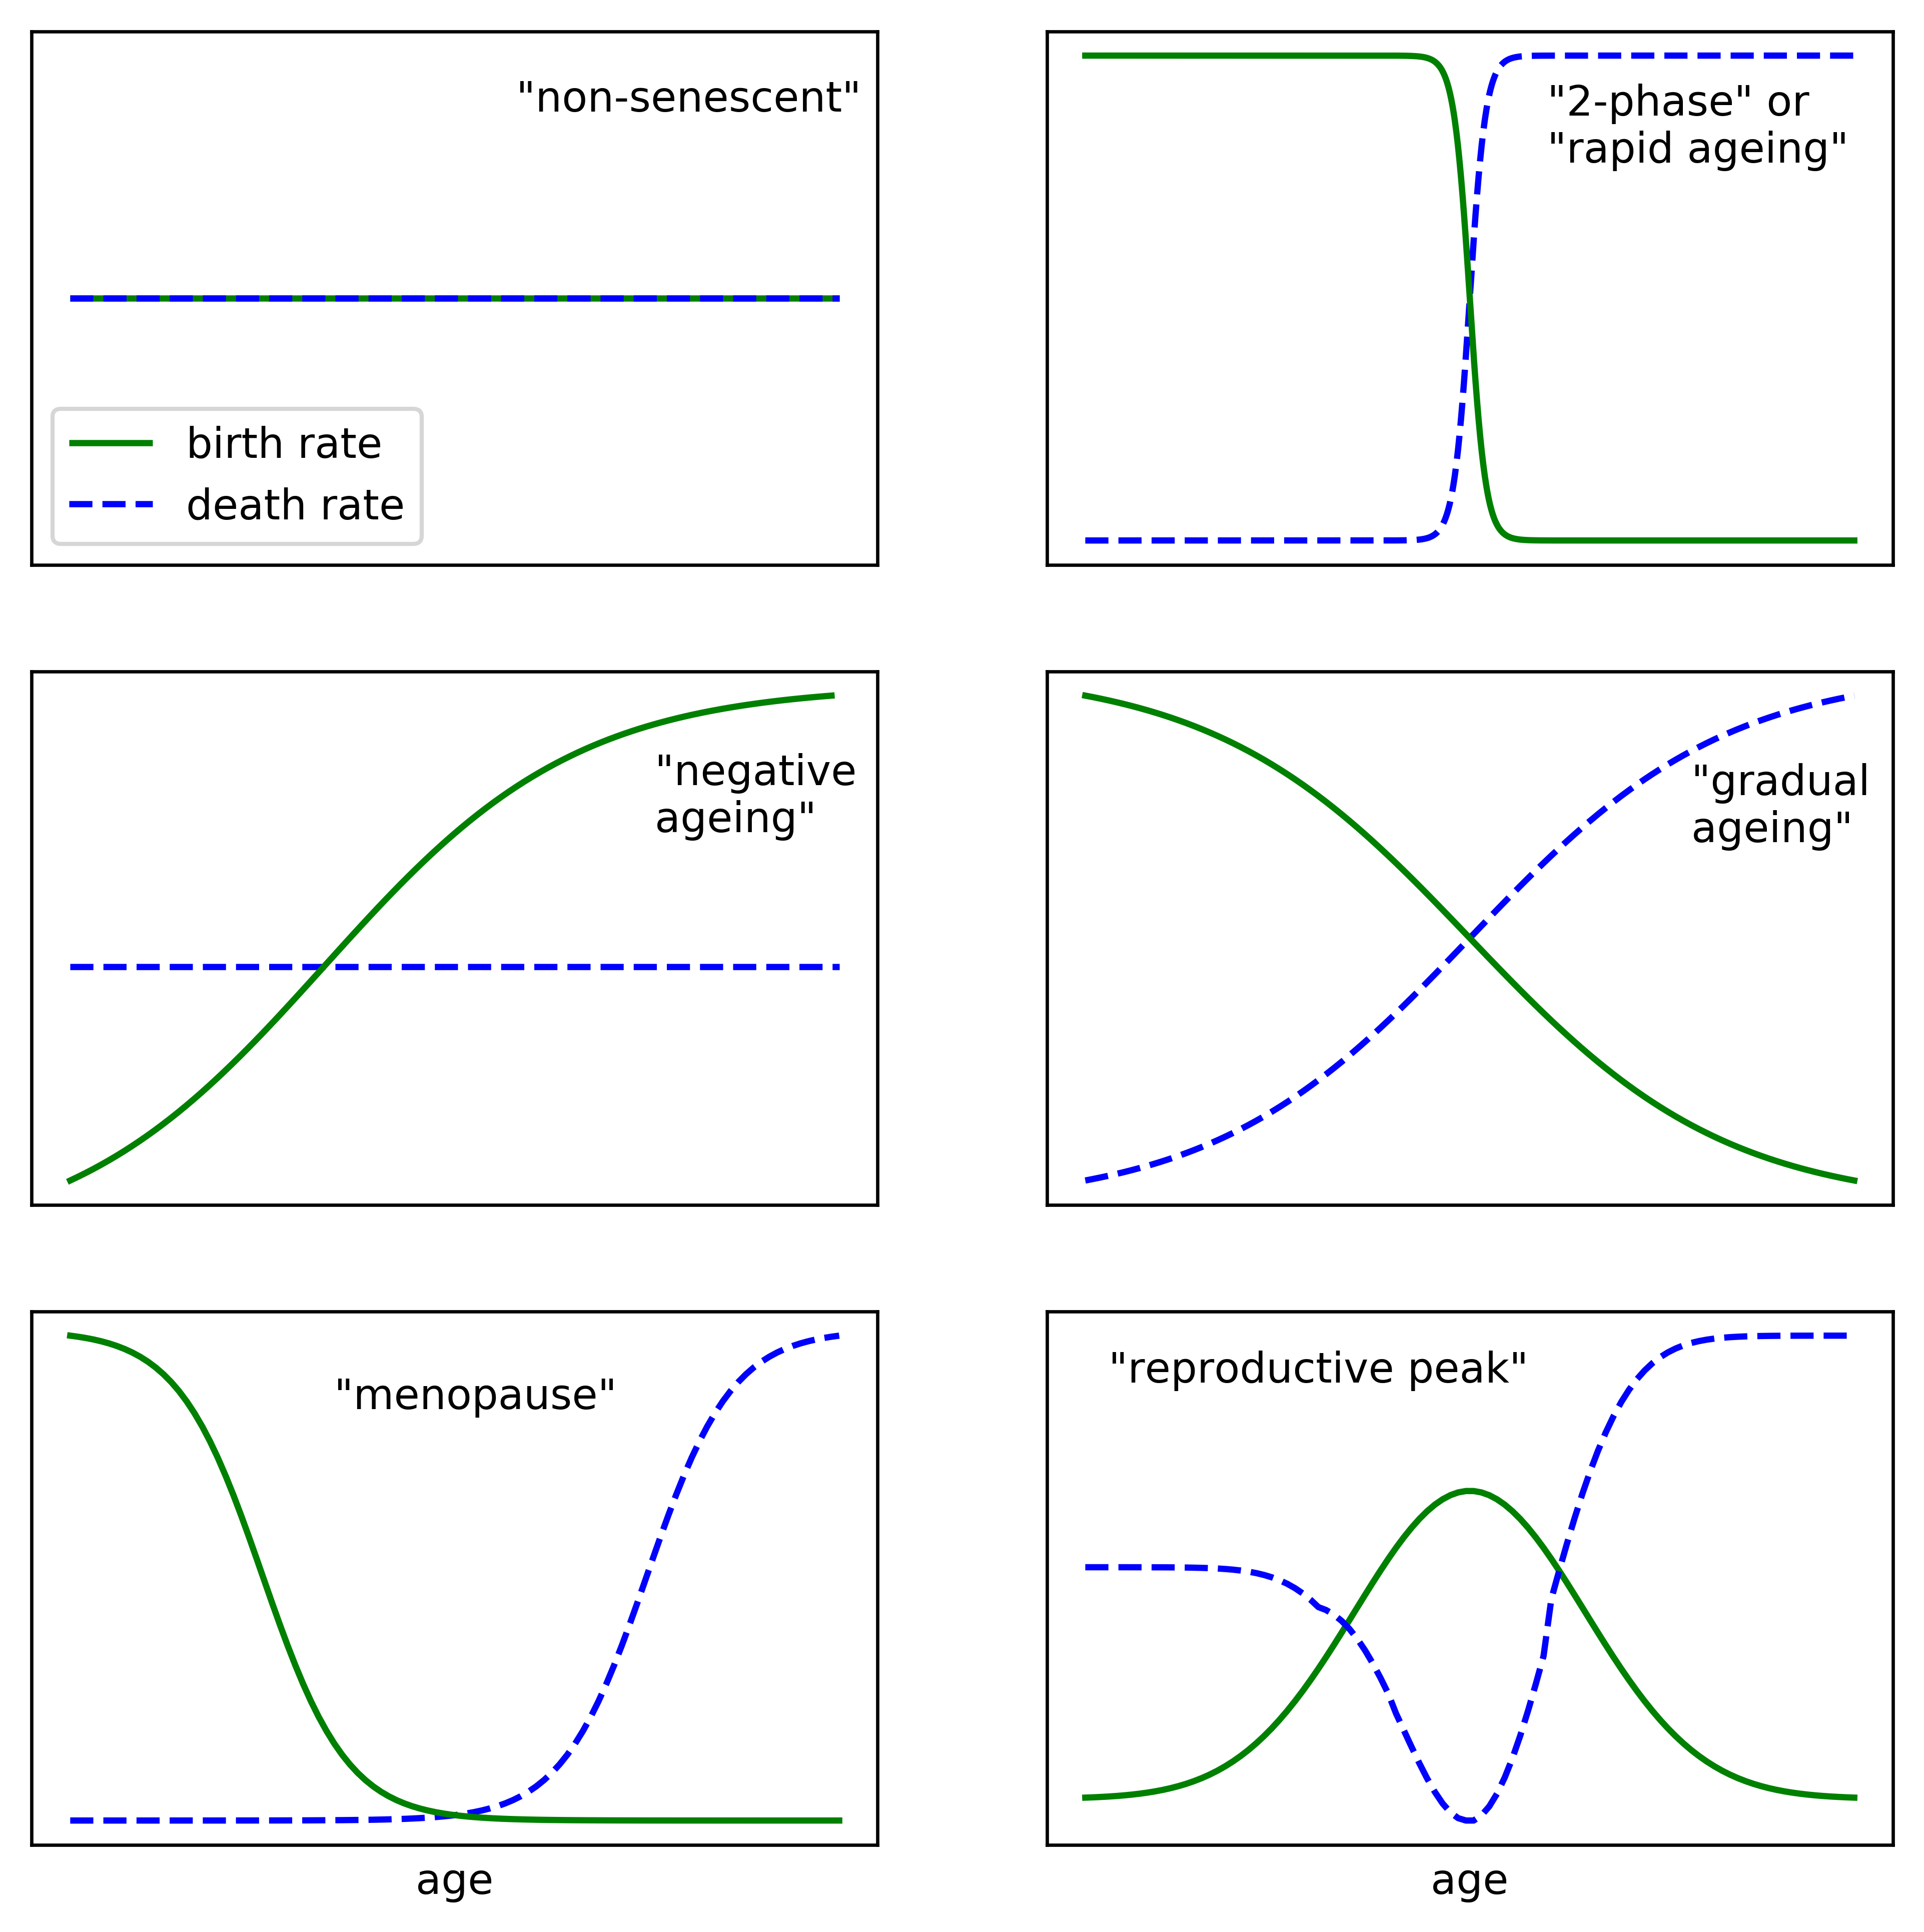
\includegraphics[scale=0.7]{figures/life-histories.png}
        \caption{Examples of possible \textbf{life-histories}, from top left to bottom right; i) non-senescent: birth and death rate do not depend on age; ii) 2-phase ageing: at some specific age organism's health rapidly deteriorates; iii) negative ageing: reproductive output increases with age while mortality remains the same; iv) gradual ageing: organism's health deteriorates gradually over many ages; v) menopause: a life period is present where health is maintained although the organism has ceased to
        reproduce; vi) birth rate reaches a peak at some age and mortality follows approximately the inverse trend. This figure only serves to illustrate the different ways in which birth and death rate can qualitatively stand in relation across different ages, and scaling for each can be different. For concrete examples see \autocite{jones2014diversity}.}
        \label{fig1}
    \end{figure}

    Following this line of thought, we naturally come to consider an individual based population structured in trait and age. If we, for simplicity's sake, restrict ourselves to a clonally reproducing population, where mutation is the only source of novel traits and mutation rate is a constant, then we can use the same approach as in section 2 to describe our model.

    The question then remains how we should parametrize birth and death rate, $b(x,a)$ and $d(x,a)$, or more precisely, how should we make them depend on the trait $x\in \chi \subset \mathbb{R}^d$ and age $a\in \mathbb{R}_+$.

\subsection{The parametrization}
    The question of parametrization is an important one, since the choice of parametrization will determine the set of possible life-histories for our model. If for instance, we take $x \in \chi \subset \mathbb{R}^4$, $\chi$ bounded, $b(x,a) = b(x_1,x_2, a) = x_1 e^{-x_2 a}$ and $d(x,a) = d(x_3, x_4, a) = x_3 (1 - e^{-x_4a})$, then we make the assumption that reproduction decreases with age and the organism becomes infertile at some late age, and that mortality increases with age and reaches a plateau at some late age. This is true for many species in nature, but instead we want a parametrization that allows us greater plasticity when investigating how such or any other life-history could evolve from an initial non-senescent one, where reproduction and mortality are constant over age.

    That is why, inspired by \autocite{sajina2016silico}, the following is proposed:
    let $\chi \subset \mathbb{R}^{2d}$ be compact and let $\tilde{\chi} := \chi \times \mathbb{R}_+$. Partition $\mathbb{R}_+$ in $d$ half-open intervals $(I_j)_{j \in \{1, \ldots, d\}}$ that we call \emph{biological ages}. Let $(I_j)_{j \in \{1, \ldots, d\}}$ be sorted ascendingly, meaning that for $I_i = [\tau_i, \tau_i'), I_j = [\tau_j, \tau_j')$ and $i<j$, it holds $\tau_i' \leq \tau_j$. Define the birth and death rate functions as:
    \begin{align}
        b(x,a) = b(x_1,\ldots,x_d,a) &= \sum_{j=1}^d \mathbbm{1}_{I_j}(a) x_j \label{eq:bstep}\\
        d(x,a) = d(x_{d+1},\ldots,x_{2d},a) &= \sum_{j=1}^d \mathbbm{1}_{I_j}(a) x_{d+j} \label{eq:dstep}
    \end{align}

    \noindent where $I_d = (a_{max}, \infty)$ is the maximum biological age for some $a_{max}>0$. Also, let Assumption \ref{ass1} hold.

    As desired, this allows for $b$ and $d$ to approximate a wide range of different life-histories that we observe in nature, but it is important to think about the biological interpretation of (\ref{eq:bstep},\ref{eq:dstep}). For this, it is decisive how we let mutation act:
    \begin{definition}\label{def1}
    \begin{itemize}
        \item[i)] mutation acts on $x$ as a whole:\\
            $x$ represents one gene whose effect determines the organism's age-specific capacity to reproduce and survive. The mutation law is $2d$-dimensional and a mutant's capacity to survive and reproduce differs from its parent's for all ages.
        \item[ii)] mutation acts on $x_{birth} := (x_1,\ldots,x_d)$ and $x_{death} := (x_{d+1},\ldots,x_{2d})$ independently:\\
            This is equivalent to having two traits. $x_{birth}$ and $x_{death}$ represent genes whose effects independently determine the organism's age-specific capacity to reproduce and survive, respectively. A newborn individual is a mutant in either $x_{birth}$ or $x_{death}$ with probability $m(1-m)$ and a mutant in both with probability $m^2$. The mutation law is $d$-dimensional.
        \item[iii)] mutation acts on each $x_j, j\in\{1,\ldots,2d\}$ independently:\\
            This is equivalent to having $2d$ traits. $x_j$ represents a gene whose effect independently of $(x_i)_{i\neq j}$ determines the organism's capacity to either reproduce ($j\leq d$) or survive ($j\geq d+1$) during exactly one biological age $I_j$ or $I_{j-d}$, respectively. A newborn individual is a mutant only in $x_j$ with probability $m(1-m)^{2d-1}$ and a mutant in $l$ fixed different traits with probability $m^l(1-m)^{2d-l}$. The mutation law is $1$-dimensional.
    \end{itemize}
    \end{definition}

    Noteworthy, in case i) a single mutation could give rise to both qualitative and temporal pleiotropy, meaning that a single gene has an effect on both qualitatively different phenotypes, namely reproduction and survival capacity, and temporally different phenotypes, namely at different ages. In this sense, in case ii) a single mutation can give rise to only temporal pleiotropy and in case iii) a single mutation can not give rise to any type of pleiotropy. Of course, in cases ii) and iii),
    multiple mutations occuring in a single birth event can give rise to a pleiotropic mutant, but in most cases the mutation rate is sufficiently small such that this is highly improbable.

Also worth remarking is that this model does not allow for any epigenetic effects (regulation of gene expression without alternations of the gene itself).

\subsection{Implications for studying ageing}
    Obviously, following our definition of ageing, the most clear example of an ageing life-history in this model would be a trait for which  $x_1$ to $x_d$ is decreasing and $x_{d+1}$ to $x_{2d}$ is increasing.
    We can stop to think about what the evolutionary theories of ageing would predict for the behaviour of the model. If we consider an initially monomorphic population with trait $x_0$ and choose $a_{max}$ (recall that the maximum biological age is $I_n = (a_{max},\infty)$) such that virtually all individuals reach $I_n$ and there is no post-reproductive life period (menopause), meaning $b(x,a) > 0$ is possible for all ages $a\geq 0$, then Fisher would lead us to believe that evolution will
    drive birth rate to its upper and death rate to its lower bound, since all ages would be under positive selection pressure. 
    
    If however, we choose $a_{max}$ such that very few or no individuals reach $I_n$, and so a "selection shadow" emerges, Medawar says that selection will drive birth and death rate to their upper and lower bounds respectively, for early biological ages, but that for ages in the selection shadow, $b$ and $d$ will maintain a higher frequency of mutations and therefore fail to reach high and low values respectively.
    Furthermore, Williams suggests that a mutant with, for instance, higher birth rate for early biological ages and lower birth rate for later biological ages than the resident, would be in selective advantage and could become fixed in the population.

    This model allows us to put all these hypotheses to test. What is more, through a specific choice of how mutation acts, we gain some degree of control as to which theory we want to test. For instance, in cases i) and ii), assuming a centered symmetrical mutation law (e.g.\ normal distribution), with the incresing number $d$ of biological ages, the chance that a mutant is either advantageous or disadvantageous for all ages compared to the resident decreases exponentially, hence virtually all mutants will represent an antagonistic trait in some sense. 
    On the other hand, in case iii), if we choose the mutation rate sufficiently low, we can guarantee that virtually all mutants will be either advantageous or disadvanageus for only one age compared to the resident, and can then investigate if this advantage is differently quantified depending on the age upon which mutation acts.
    
    If we were to analyze this model in the adaptive dynamics limit, obtaining the equivalent of equation \eqref{eq:estprob} would allow us to ask how the establishment probability of a mutant in a resident population depends on the mutation. More precisely, if it is higher for mutations that increase fitness for early ages compared to those that increase it for later ages and to what extent can a trade-off occur in the sense that a mutant with increased early-life and decreased late-life fitness successfully invades.
    This would in a sense quantify the force of natural selection depending on age and it would address the antagonistic pleiotropy theory, namely that an ageing phenotype could evolve through a trade-off favoring early fitness.

    Admittedly, the here step-functions of age, $b$ and $d$, violate Assumption \ref{ass2} i). Furthermore, when choosing how mutation acts, only case i) from Definition \ref{def1} stays consistent with what we have described in section 2. For cases ii) and iii) from Definition \ref{def1} we would get additional terms for different possible mutants. Trying to derive TSSage and CEAD for this model therefore requires work. This is not pursued in this thesis.

    On the other hand, simulating this model numerically is straight-forward, the underlying concept being described in section 2.1. One can first start simulating a monomorphic population under rare mutations. With a large enough population size, \eqref{eq:supercrit} should be a relatively good guideline for finding parameters under which a stable age distribution is obtained. The first test would then be too see if the model can evolve an ageing phenotype. This is pursued in the remainder of this section. Finally, one would in a more systematic manner explore the "parameter space", or in other words, draw a map of which sets of parameters most likely lead to which outcomes.

    %However, because of the separation of time scales and the resulting process that moves from one successfull mutant to the other, with adaptive dynamics we cannot address Medawar's theory that mutants that are not advantageous and carry a deleterious mutation acting in a late age would persist in the population.
    
    %What we can not address in the adaptive dynamics limit is the role of genetic drift in the evolution of traits, since genetic drift occurs in populations of finite size. Moreover, we can not investigate how frequent mutation can weaken selection effectiveness.

    %Here the numerical simulation comes to rescue, with help of which we can observe and try to identify which of the above mentioned selective mechanisms are taking place. For the scenario without selection shadow, any ageing phenotype evolved would have to be ascribed to antagonistic pleiotropy. For the scenario with a selection shadow, later ages frequenting at rates that we would expect for a neutrally evolving trait would correspond to mutation accumulation, while later ages frequenting at lower than neutral rates would indicate that antagonistic pleiotropy has taken place.

\subsection{Numerical simulations}
    We are interested in simulating the above described model and seeing to what extent the model's behaviour is predicted by evolutionary theories of ageing. To that purpose, the model was implemented in Python, following the construction concept of section 2.1. This section presents figures for data obtained from the simulations, portraying different aspects of the model's behaviour: trait configuration of the final population, age distribution, population size and the evolutionary trajectories
    of traits. The choice of parameters is firstly listed and then the figures are commented.
    
    Before simulating, we need to choose how mutation will act and come to a choice of parameters that describe the biological features of the population. For brevity, here only cases ii) and iii) from Definition \ref{def1} will be considered for how mutation acts. The following is true for all simulations presented in this section:
    \begin{itemize}
        \item The starting population size is $10^4$.
        \item The starting population is monomorphic with birth rate $b_0 = 2.0$ and death rate $d_0 = 1.5$ and all individuals in the starting population are born at time $t=0$ (i.e.\ start with age $0$).
        \item The upper bound for birth rate is $\bar{b} = 4.0$ and the lower and upper bounds for death rate are $\ubar{d} = 0.1$ and $\bar{d} = 4.0$ (recall Assumption \ref{ass1}).
        \item The competition kernel $c((x,a),(y,\alpha))$ is a constant $\eta = 5\cdot 10^{-5}$.
        \item The mutation rate is given by $m = 10^{-2}$.
        \item The mutation law $M(x,dh)$ is a centered normal distribution with variance $\theta^2$.
        \item There are $11$ biological ages, which divide the interval $[0, a_{max})$ in $10$ intervals of same length, where $a_{max}$ is the maximum age, and the $11$th biological age is the interval $[a_{max}, \infty)$.
        \item The number of simulated jumps is $2\cdot 10^6$.
    \end{itemize}

    \noindent Note that the choice of the competition kernel as a constant means that every individual exerts the same environmental pressure on any other individual, independent of their traits or ages. In particular, at each time $t$, the death rate of an individual with trait $x$ and of age $a$ will amount to $d(x,a) + N_t \eta$, where $N_t$ is the population size at time $t$. Furthermore, keep in mind that the mutation rate $m$ is defined per trait and therefore its
    interpretation depends on how mutation acts (see Definition \ref{def1}).

    The reader will notice that three parameters remain unspecified:
    \begin{itemize}
        \item[1)] Does mutation act as in case ii) or as in case iii) (see Definition \ref{def1})?
        \item[2)] What is the "severity" of mutations $\theta$?
        \item[3)] What is the maximum age $a_{max}$?
    \end{itemize}

    \noindent It is these three parameters that we will vary to see if and how the model's behaviour changes. In the following, we will call simulations in which mutation acts as in case ii) "2trait", and mutations in which mutation acts as in case iii) as "single". $\theta$ takes values $0.25, 0.50, 1.00$ and $a_{max}$ is either $2.0$ or $5.0$.

    Figure \ref{fig:agedist} helps us motivate the choice of maximum age $a_{max}$. We see that for $a_{max} = 5.0$ the population is concentrated in the first few biological ages, while virtually no individual reaches later biological ages. In case $a_{max} = 2.0$ however, we see that a larger proportion of individuals reaches intermediate and late biological ages. Therefore this choice results in an age distribution that suggests a greater "selection shadow" is present in case $a_{max} = 5.0$.

    \begin{figure}[!htb]
        \center
        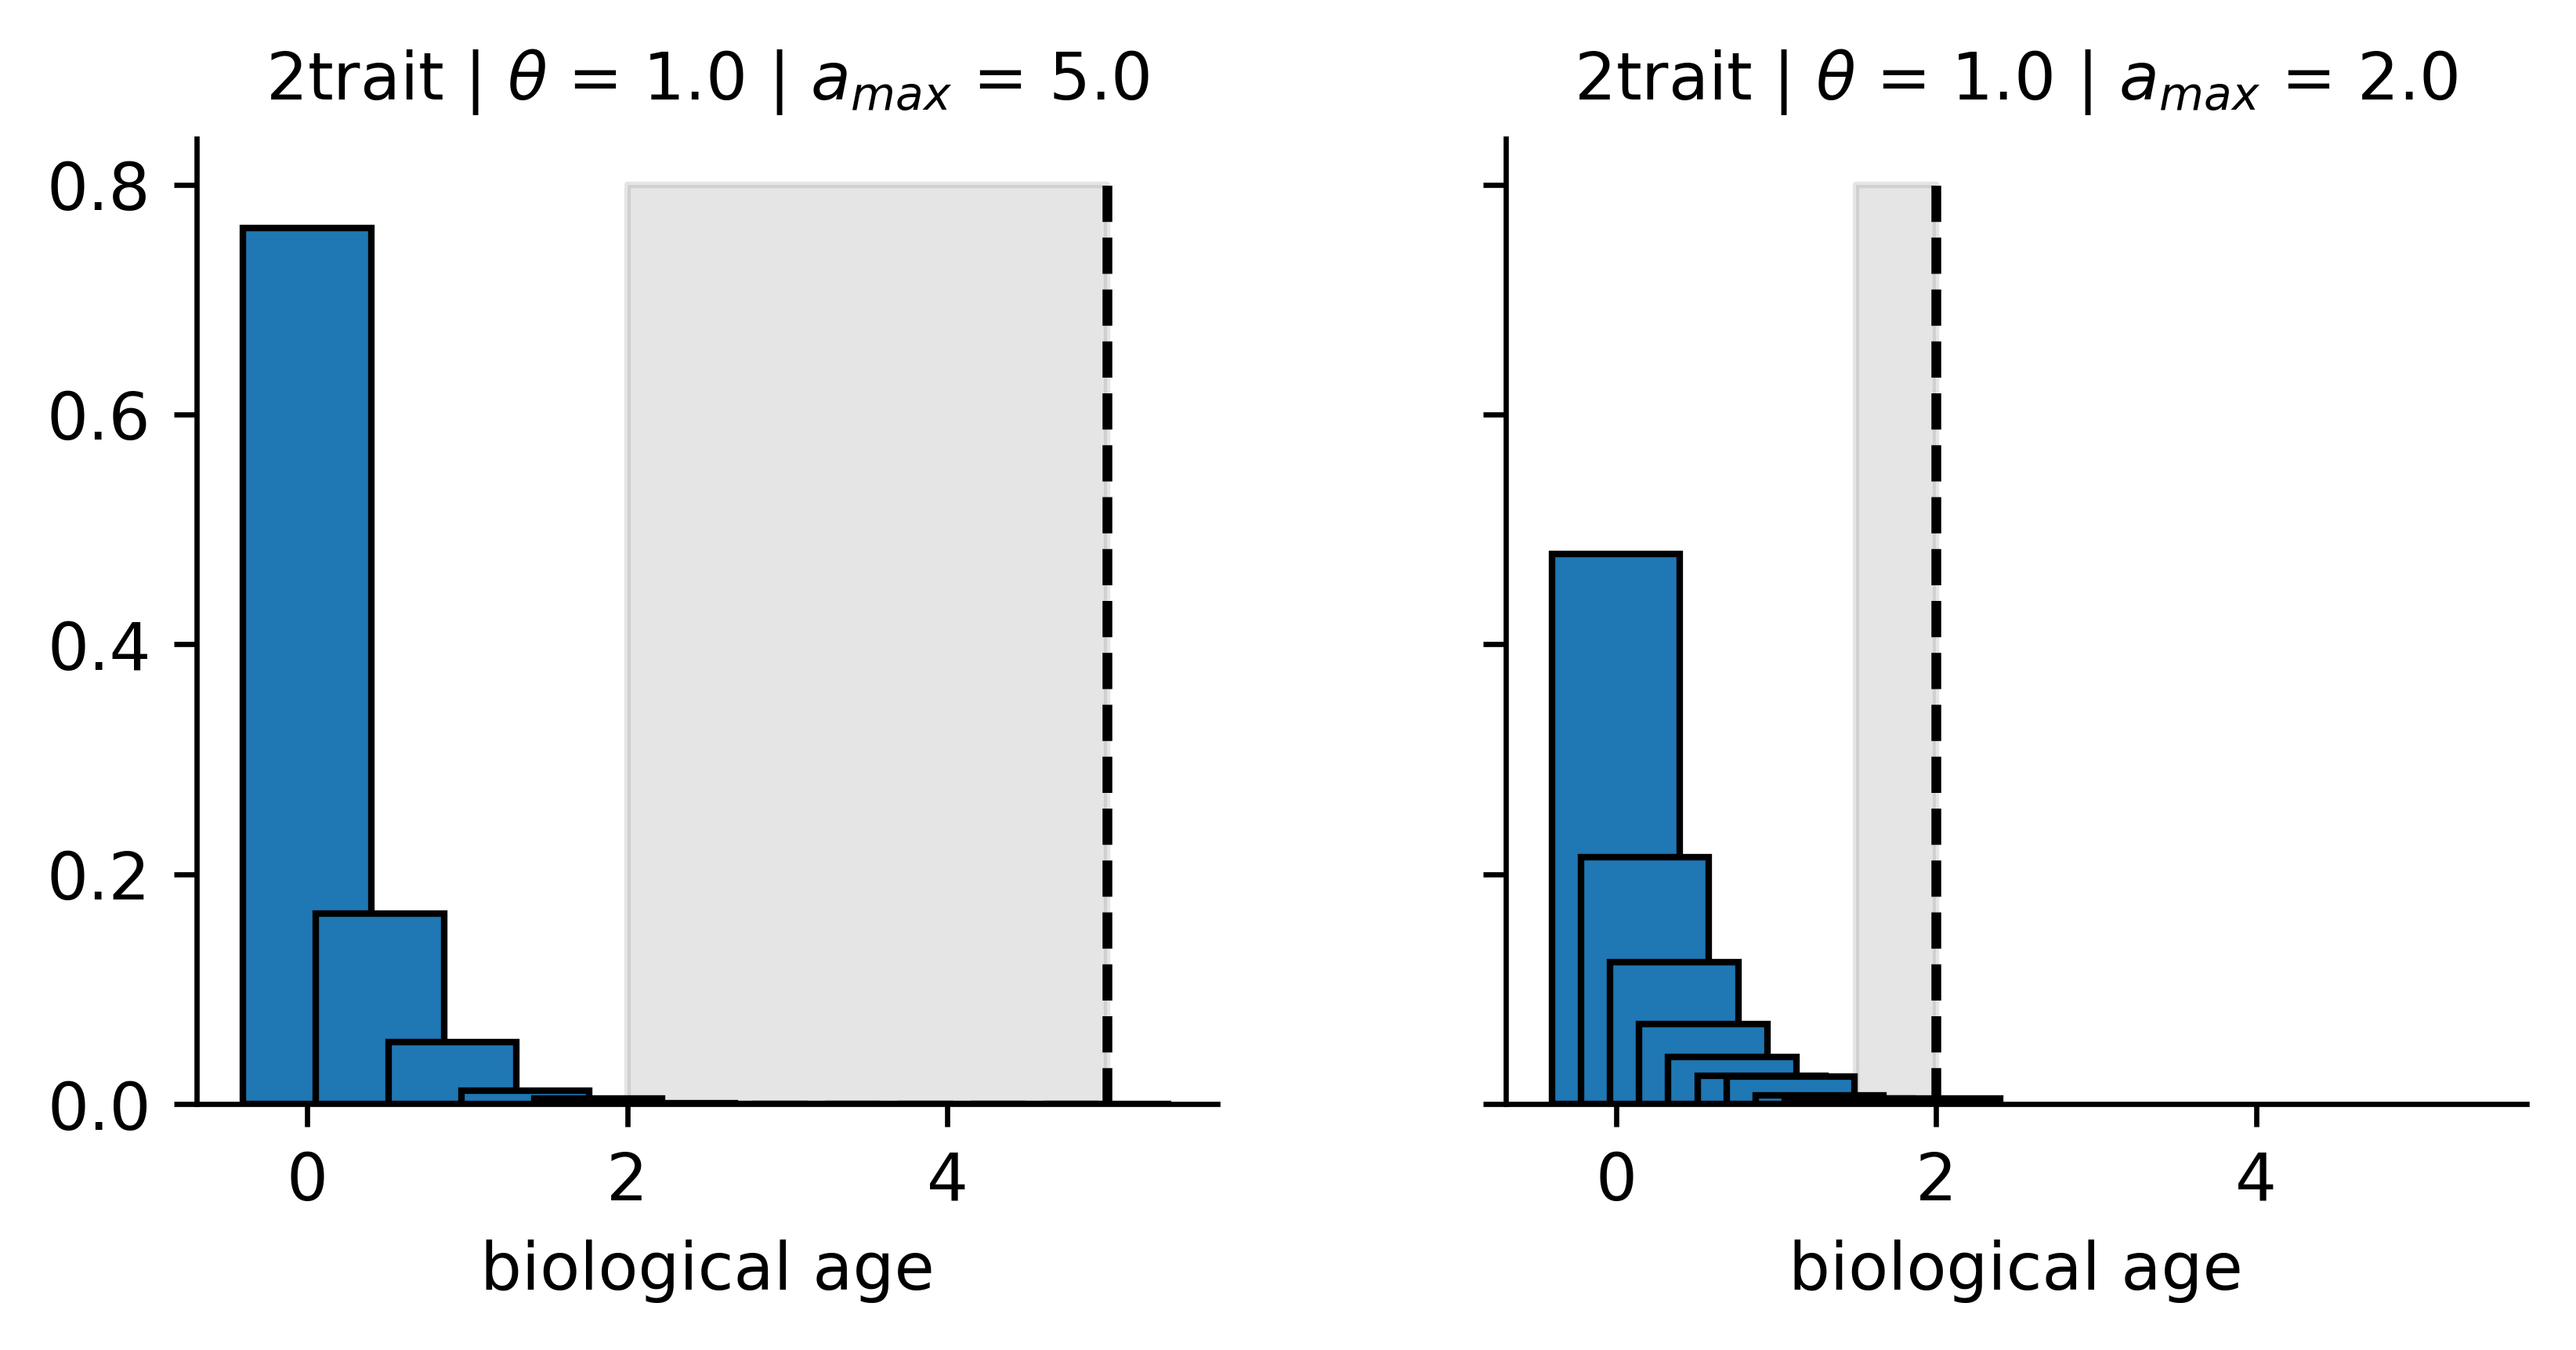
\includegraphics[scale=0.8]{figures/age_dist.png}
        \caption{\textbf{Age distribution} is shown for two simulations differing only in maximum age $a_{max}$. The bars represent the proportion of individuals for different discrete biological ages. The data was sampled for ten equidistant timepoints between time zero and the time of the last jump, and averaged. For clarity, the biological ages in case $a_{max}=5.0$ are the intervals $[0,0.5), [0.5,1.0), \ldots, [4.5, 5.0), [5.0, \infty)$. For $a_{max} = 2.0$ it is $[0,0.2), [0.2,0.4), \ldots, [1.8,
        2.0), [2.0, \infty)$. The dashed vertical lines indicate the maximum age and the shaded area refers to the "selection shadow". Both simulations are "2trait" and have $\theta=1.0$.}
        \label{fig:agedist}
    \end{figure}

    Recalling the expectations for this model's behaviour that arise from evolutionary theories of ageing (see section 3.2), we would therefore expect to see patterns of positive selection for more biological ages when $a_{max}=2.0$. Furthermore, we would hold it more likely for "2trait" populations to evolve deleterious late-acting traits. Figure \ref{fig:step} shows the mean birth and death rate for a population after $2\cdot 10^6$ jumps, for all possible combinations of the parameters that we are varying.

    Indeed, we see that in no simulation is the fitness maximized, and all simulations consistently evolve elevated birth rates and low death rates only for the first few biological ages. Furthermore, we see that for simulations with $a_{max}=5.0$ this observation is restricted to the first two ages, while for simulations with $a_{max}=2.0$ this tendency extends up to the fifth age.
    Going further, we see that in "single" simulations the rates for later ages stay in the neighbourhood of their initial values, while this is far more volatile for "2trait" populations. Finally, we see that with growing mutation severity $\theta$, the birth and death rates reached for early ages are higher and lower, respectively, and that the mentioned volatility effect is stronger.

    \begin{figure}[!htb]
        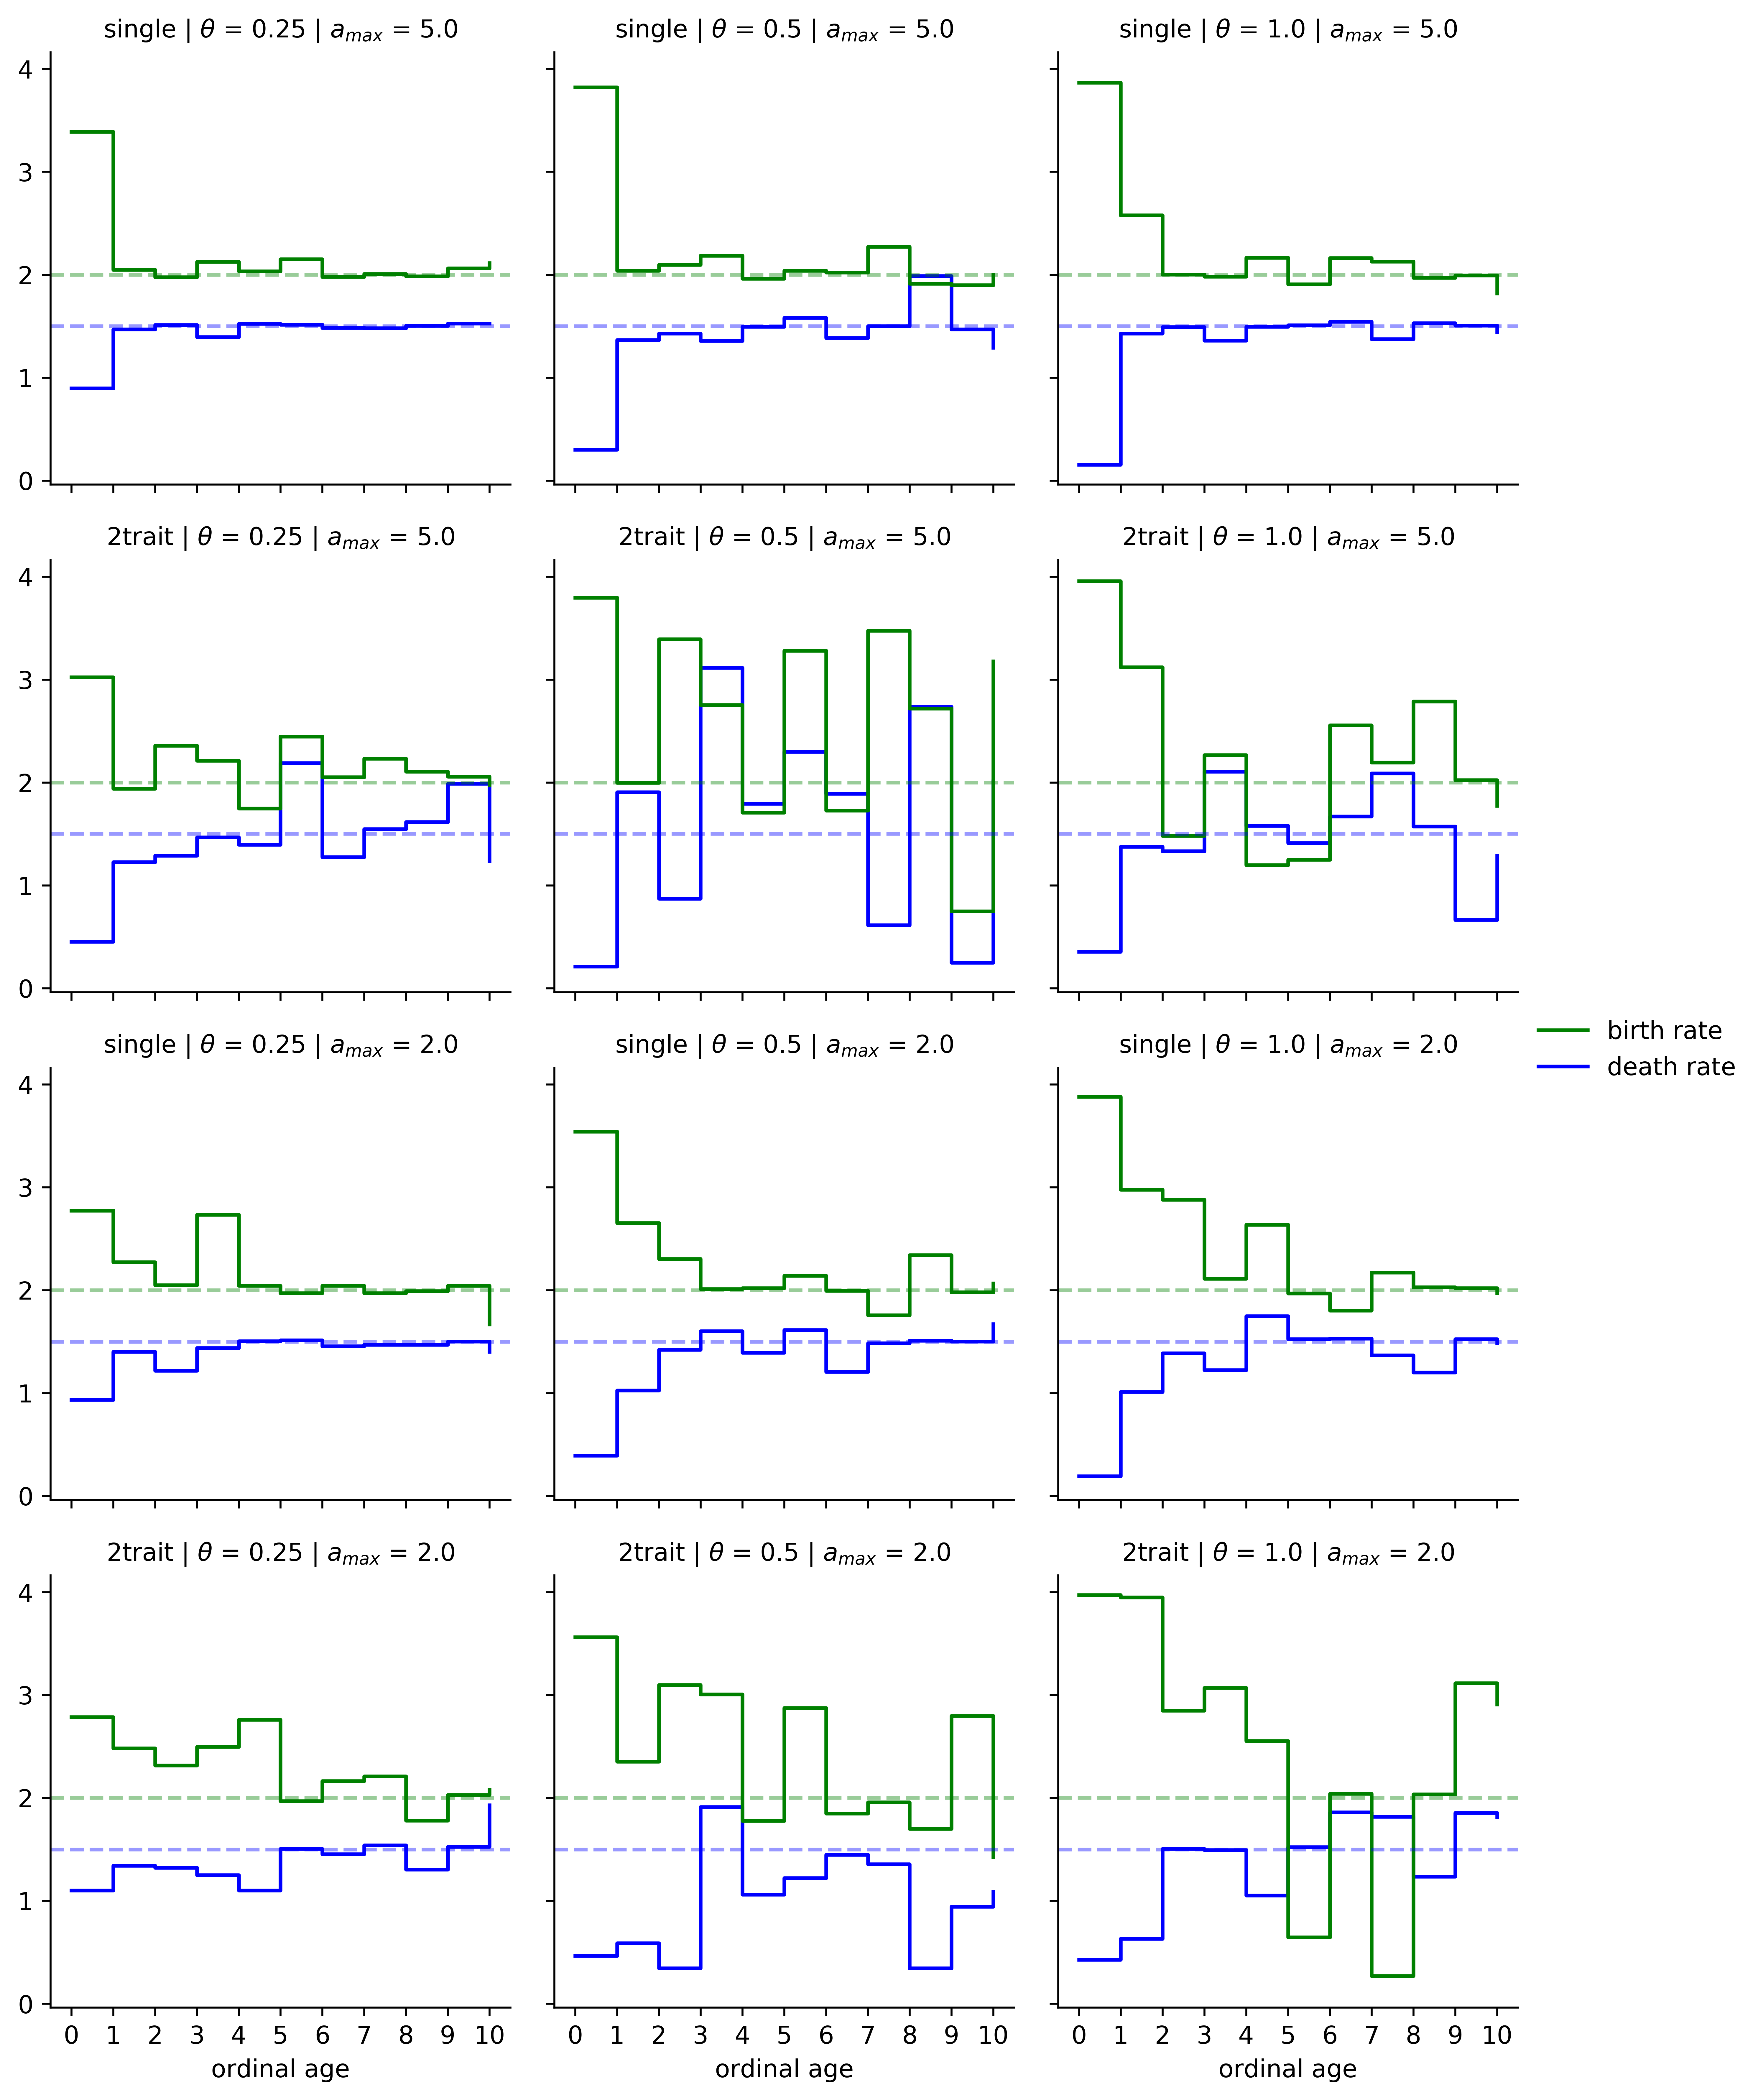
\includegraphics[width=\textwidth]{figures/step-mage_5_2.png}
        \caption{\textbf{Final states} for birth and death rates under different parameters after $2\cdot 10^6$ simulated jumps are shown. For representation purposes, the x axis is in ordinal age, by which we simply mean the ordinal number of the respective biological age for either $a_{max}=5.0$ or $a_{max}=2.0$. The dashed horizontal lines indicate the initial values of the rates. The captions above each axes indicate the varied parameters of the simulation.}
        \label{fig:step}
    \end{figure}

    Figure \ref{fig:traits} better reveals the effect of changing $\theta$. Here we see, exemplary for the birth rate, that with higer values of $\theta$ the rate for ordinal age $0$ reaches the neighbourhood of the upper bound in fewer jumps. Moreover, the greater $\theta$ is, the greater the spread of the most of the other ordinal ages.

    \begin{figure}[!htb]
        \center
        \includegraphics[width=\textwidth]{figures/trait_evo2.png}
        \caption{\textbf{Trait evolutionary trajectory} is shown for birth rate and simulations with $a_{max}=5.0$. The lines show how the mean population birth rate has changed over 10 equidistant timepoints between time zero and the time of the last jump. The line colors indicate to which ordinal age (ordinal number of respective biological age) the lines correspond to.}
        \label{fig:traits}
    \end{figure}

    This phenomenon is reflected when we look at how population size changes with time. Figure \ref{fig:popsize} shows us that higher mutation severity $\theta$ leads to a faster evolution of population size toward its carrying capacity. Only sometimes, everything else being equal, does population size in "2trait" simulations grows faster than in "single" simulations.

    Indeed, there is no reason to believe that, all else being equal, "2trait" simulations are somehow better than "single" ones in producing the phenotype at age zero for which we see a selective pattern in Figure \ref{fig:traits}, and which ultimately leads to the expansion in population size. As mentioned before, the mutation rate $m=10^{-2}$ is to be interpreted differently for "2trait" and "single" simulations. In "2trait" simulations, it means that on average $1-(1-m)^2 \approx 2\%$ births are mutants, and every
    mutant has birth or death rate different from its parent, \emph{for all ages}. In "single" simulations, it means that on average $1 - (1-m)^{2n_{age}} \approx 20\%$, where $n_{age} = 11$ is the number of biological ages, of
    births are mutants for birth or death rate for at least \emph{one age}, but only $2m \approx 2\%$ of  births are mutants for birth or death rate for age zero. Hence, on average, "2trait" and "single" populations should produce this phenotype at the same rate. In "2trait" populations however, a mutant is more likely to be advantageous for multiple ages, and this aggregate effect could explain why we occasionally see more rapid selection in this setting.

    \begin{figure}[!htb]
        \center
        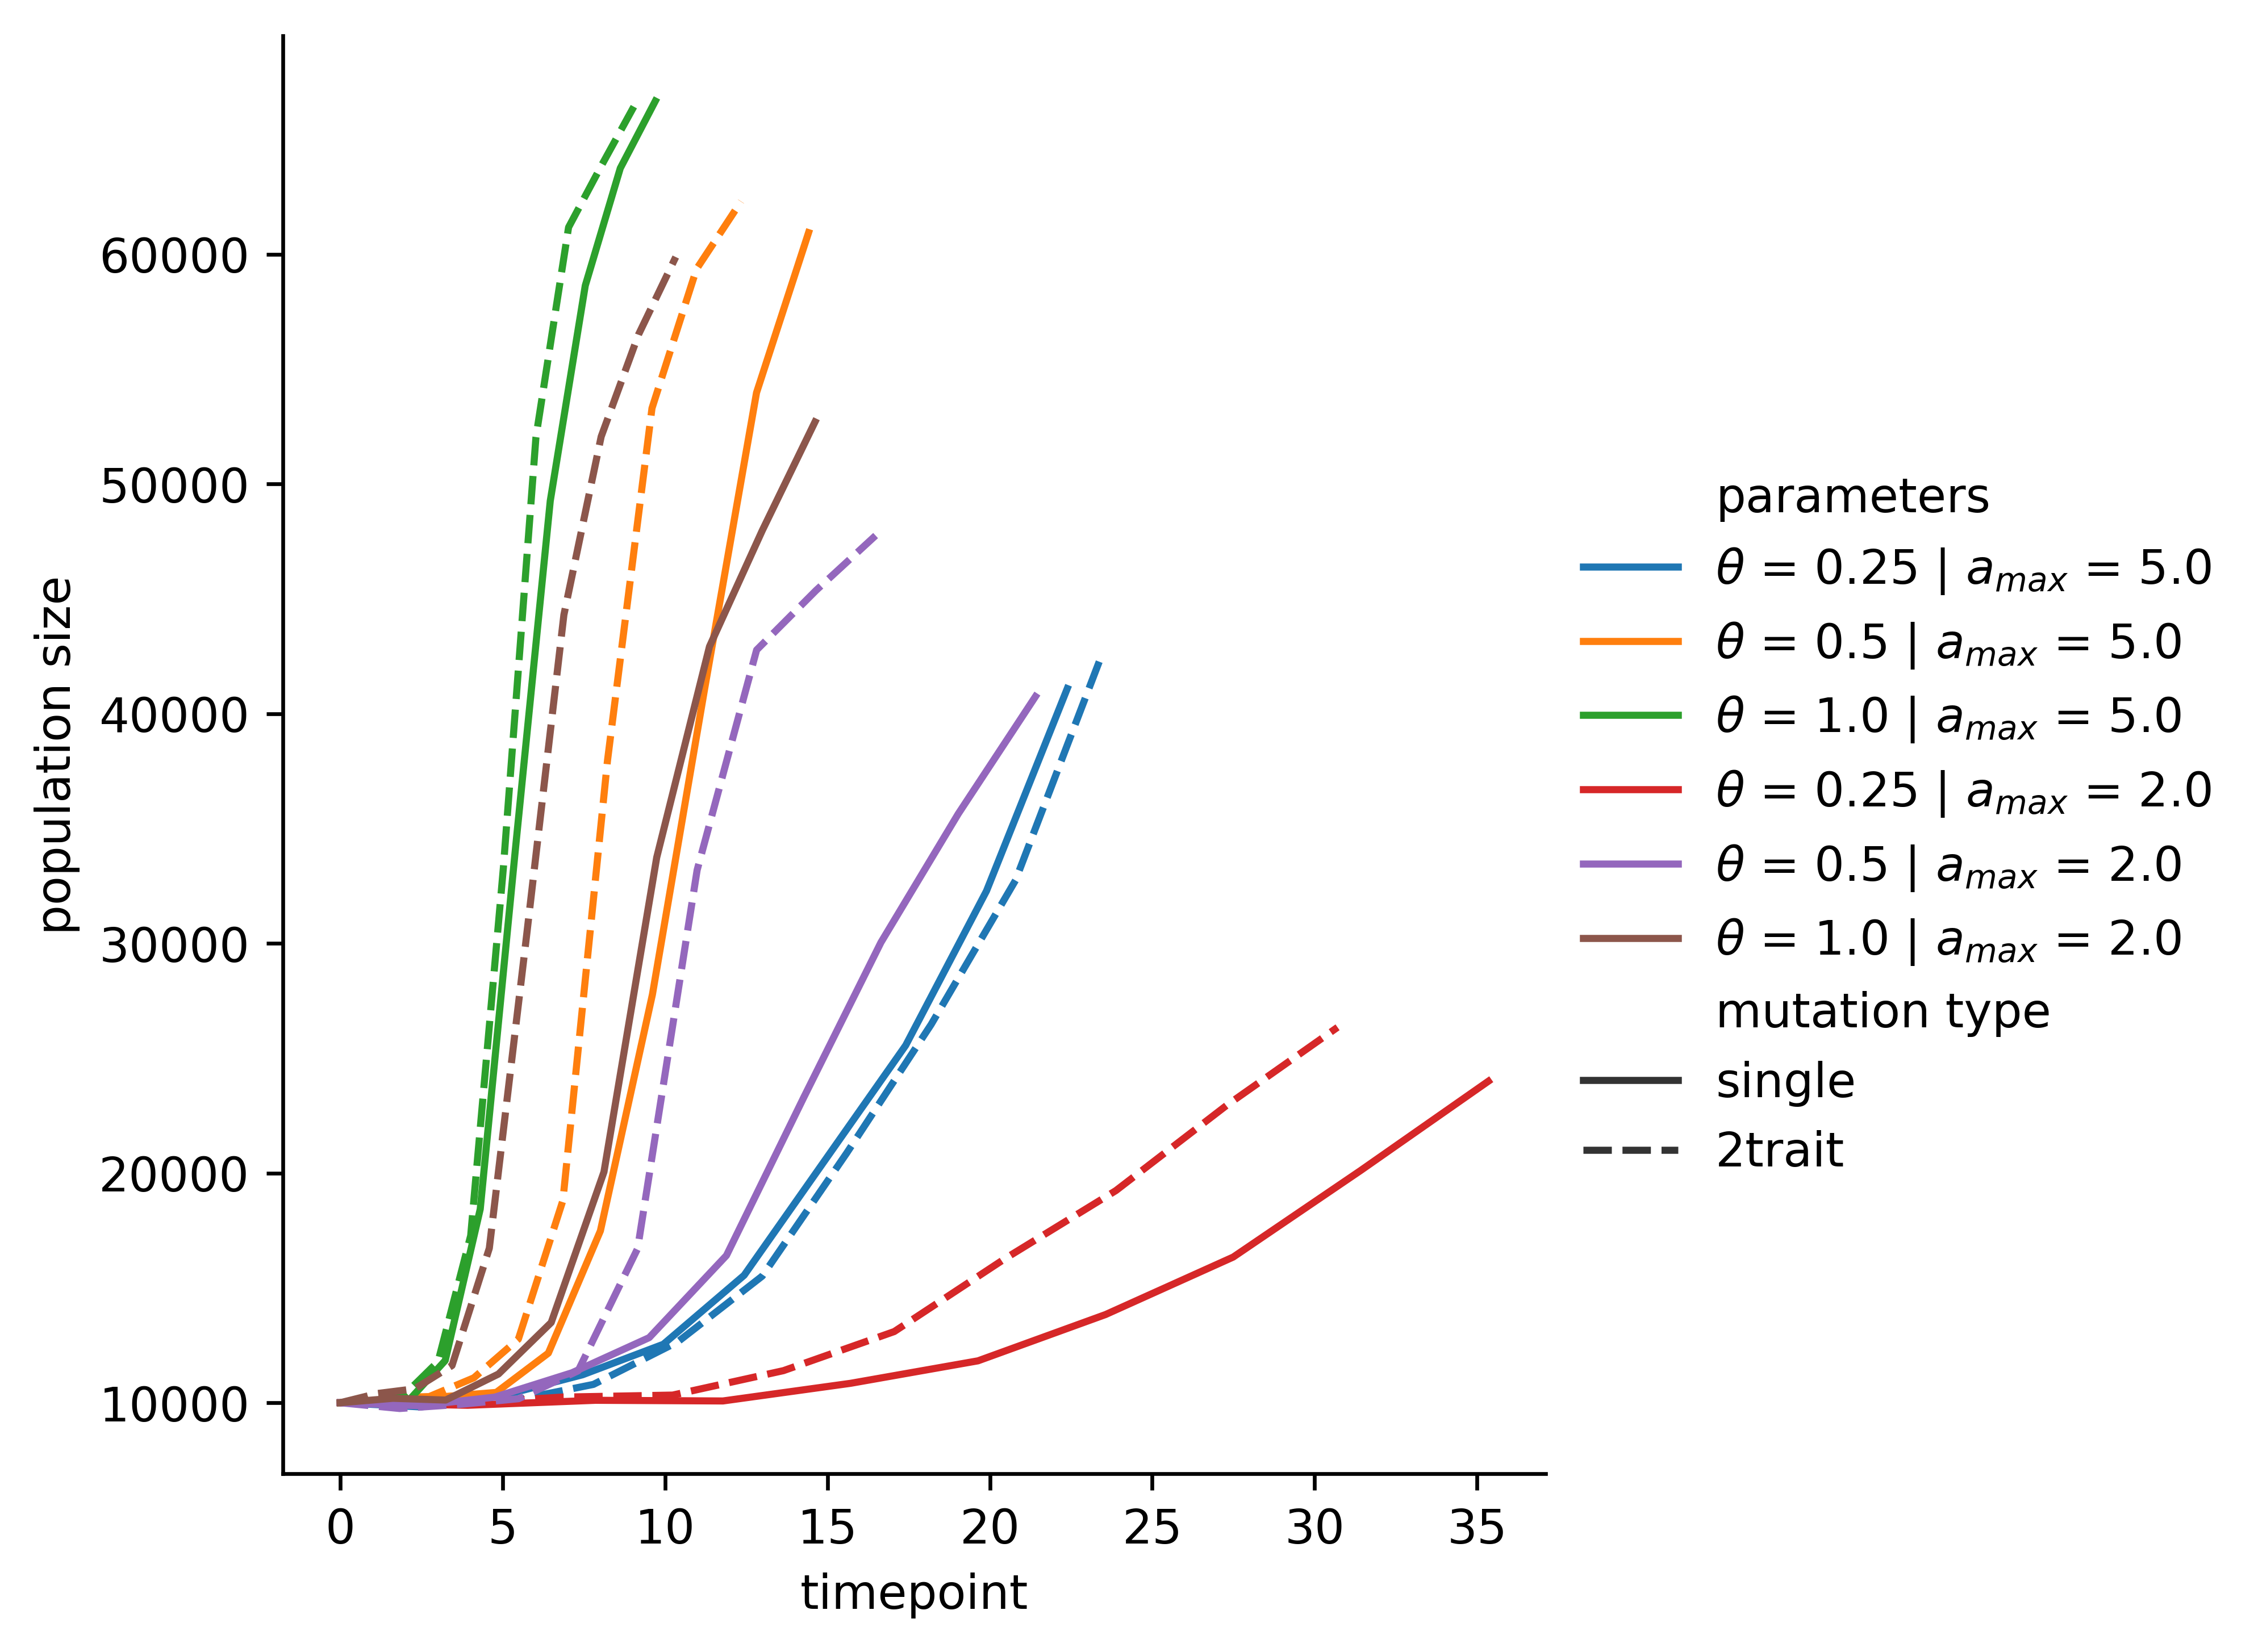
\includegraphics[scale=0.6]{figures/population_size.png}
        \caption{\textbf{Population size} is shown under different simulation parameters. The lines show how population size has changed over 10 equidistant timepoints between time zero and the time of the last jump. The line colors indicate to which simulation the lines correspond to. Furthermore, "single" simulations are drawn with a full line, while "2trait" simulations are drawn with a dashed line.}
        \label{fig:popsize}
    \end{figure}

    Turning our attention to Figure \ref{fig:step} again, we can revisit the motivating question of this model: do we see evolution of ageing phenotypes? Recalling the definition of ageing as an increase in death rate and a decline in birth rate with age, we can argue that indeed, this model in its simple form, can recapitulate this phenomenon. Moreover, we see that in "single" simulations, where mutations are not pleiotropic, evolution drives only traits affecting early ages to
    values of higher fitness, while the remaining traits remain in the neighbourhood of their initial values. On the other hand in "2trait" simulations, when we allow pleiotropic mutations, evolution of high early age fitness can be related to lower-than-initial-state fitness for later ages. 

    



%\subsubsection{Detecting selection and relaxation patterns}
%    For the specific choice of parameters made in the simulations, we are interested in the long-term behaviour of the average value of some neutral locus $L$ with initial value $x_0\in\mathbb{R}_+$, or concretely in its expected value and variance after the population has made $n\in\mathbb{N}$ jumps. If we can say something about it, we can compare how similar or different  the behaviour of other loci is, and therewith obtain an indicator for which loci are likely to be under selection or evolving neutrally.
%
%    Without further restrictions, this problem is hard, because the number of mutations in the whole population that occur on locus $L$ in the course of $n$ jumps depends not only on the mutation rate, but also on birth and death rates of all living individuals. One cop-out is to run the simulations sufficiently often and check that the same results are repeatedly obtained.
%
%    Another one is to add a neutral locus to the model and use it as a reference point for neutral evolution. In the short term, this approach is susceptible to a 'hitchiking effect', meaning that some advantageus mutant goes to fixation, so will the specific value of the neutral locus that is present in it, although the neutral locus itself did not provide the advantage. In the long term however, once the population has reached an evolutionary stable state, this locus should be a faithful representation of neutral evolution.
%
%    However, by means of further assumptions, we want to derive an approximation for the solution of this problem, so as to at least provide a validation for our cop-out, if the two approximations yield values in the same range.
%
%    Let us consider a monomorphic population whose individuals reproduce and die at rates $b,d \in \mathbb{R}_+$ for all ages, meaning that we can forget about age-structure for the moment. Also, let $b\approx \hat{d}$, where $\hat{d}$ is a death rate accounting for both the intrinsic death rate $d$ and competition between individuals, so that population size stays rougly the same across many jumps. Let us assume further that there is no mutation, except for a neutral locus $L$, with initial
%    value $x_0\in\mathbb{R}$ that undergoes mutation at each clonal birth with rate $u\in(0,1]$. Since $L$ is neutral, this means that the population will remain monomorphic at all times, because mutations on $L$ will not alter $b$ and $d$. Finally, with population size being approximately $N\in\mathbb{N}$, consider the average value of the neutral locus $L$ after $n$ jumps:
%    \begin{equation}
%        L_n = \frac{1}{N} \Big( Nx_0 + \sum_{i=1}^{K_n} X_i \Big),\quad X_i \sim N(\mu, \phi^2)~iid,
%    \end{equation}
%    where $K_n$ denotes the total number of mutations that have ocurred on locus $L$ after $n$ jumps.
%
%    $K_n$ is a random variable that depends on mutation rate, population size and the birth rate $b$. Since $L$ is neutral and therefore mutations $X_i$ do not alter how individuals reproduce or die, $(X_i)_i$ and $K_n$ are independent. Therefore we get by Wald's identity:
%    \begin{equation}
%        Var[L_n] = \frac{1}{N^2} (E[K_n]Var[X_1] + E[X_1]^2Var[K_n]).
%    \end{equation}
%    Choosing $\mu = 0$, the second term vanishes. We can approximate $E[K_n] \approx \frac{b}{b+d}Nun \approx \frac{1}{2}Nun$.
%    Hence we get $Var[L_n] \approx \frac{1}{2N}un\phi^2$. Plugging in the parameters from simulations: $N=10^4, \phi^2=0.25, u=0.01, n=10^6$, yields $Var[L_n] \approx 0.353553^2$.

    

    %As described in the introduction section about population genetics, it is highly unlikely for a mutant to attain high frequencies in the population by chance alone. Moreover, the probability that a phenotype gets fixed in a population by drift alone goes to zero as the population size goes to infinity. Therefore when such event does happen, it is safe to assume that done its part on this phenotype's behalf.

    %In our setting, it is much more straight forward to track the average traits than individual lineages. We therefore at first don't want to look for fixation events, but rather for unusually high or low average trait values, and take these events as an indicator that selection is acting. How can we specify \emph{unusually}?

    
\section{Discussion}
    When we want to investigate the evolution of ageing, we naturally come to consider an age and trait structured population. Furthermore, for a clonally reproducing population, we want to assume that there is an underlying stochastic process imitating mutation that creates the variation of traits upon which selection can act.
    Concepts from population dynamics, population genetics, evolutionary biology and finally adaptive dynamics bring us a long way in this direction, but nonetheless have their limitations.

    Adaptive dynamics for age and trait structured populations as described in \autocite{meleard2009tss} is very powerful in the sense that we can obtain information about the evolutionary trajectory of the traits under the adaptive dynamics limit, and the concept of invasion fitness allows us to ask questions like: how does the probability of fixation or elimination by selection of some trait depend on its age of expression? Still, this may only partially or not at all be applicable when
    population sizes are small or unstable.
    This is unfortunate, since there is observational support that population bottlenecks are connected to increased frequencies of gene variants that are well known to be regulators of lifespan \autocite{ray2019}.

    Moreover, the time scale separation used in this approach entails the assumption that mutations are sufficiently rare so that the population always reaches its monomorphic equilibrium between invasion events. The question remains what is different when mutations are more frequent and there are many mutants present in the population at all times.

    Conversely, numerical simulations allow us to address these issues, but often at the expense of analytical results about long-term population behaviour. With numerical simulations we therefore run the risk that our observations are an artifact of our choice of parameters. Hence, simulations boil down to intelligent experimentation and results obtained unavoidably contain some underlying uncertainty.

    The purpose of this thesis is therefore to restate the individual based model of adaptive dynamics with age structure, draw attention to a specific parametrization of birth and death rate and argue why this parametrization is suitable for studying the evolution of ageing in both the context of adaptive dynamics and numerical simulations.
    The parametrization of birth and death rate as step-functions of discrete ages allows the model to freely evolve a wide range of possible life-histories, which therefore become emergent properties of the model, rather than artifacts of the parametrization itself. Furthermore, the model can be utilized to study under which criteria do ageing phenotypes evolve, and when they do, distinguish which evolutionary theory of ageing best explains it by testing for different mutation mechanisms.

    Results from simulations suggest that ageing-like life-histories indeed can evolve in this model from an initially non-senescent one. Furthermore, we observe that firstly, higher mutation "severity", i.e.\ the average distance in trait space between the mutant and the parent, leads to a more rapid population growth, and secondly, antagonistic phenotypes are more likely to evolve when mutation acts on a gene that affects some trait for the entire lifespan of the organism, compared to mutation acting on a gene that affects some trait only for one specific biological age.
    In addition, we can theorize that due to Medawar's concept of "selection shadow", age distribution in the model is suggestive of the force of selection acting at different ages.

    The purpose of this thesis is therefore to, on the one hand, draw attention to a model that allows for adaptive dynamics to question the role of adaptive mechanisms in the evolution of ageing, and on the other hand, through numerical simulations, make us vary of the role that non-adaptive mechanisms, such as mutation accumulation and antagonistic pleiotropy, have in the evolution of ageing when the assumptions of adaptive dynamics do not hold.

    In a recent publication \autocite{meleard2018bd}, the individual-based model of adaptive dynamics with age structure was applied to model the evolution of ageing. The authors consider a clonally reproducing haploid population characterized by age and two traits: $x_b\in \mathbb{R}_+$ governing birth rate and $x_d\in \mathbb{R}_+$ governing death rate. In their model, an individual of age $a$ and with traits $(x_b,x_d)$ reproduces with rate one while $a\leq x_b$ and ceases to reproduce when $a>x_b$.
    Similarly, the individual cannot die as long as $a\leq x_d$ and dies with rate one when $a>x_d$. The two traits therefore define the duration of the organism's ability to reproduce and stay alive.
    In addition, the Lansing effect is assumed. The Lansing effect is the epigenetic effect through which the offspring of old parents has shorter life expectancy than offspring of young parents.
    The authors then proceed to show that in the adaptive dynamics limit, this model evolves to a life-history described as "2-phase" ageing (see Figure \ref{fig1}), or more precisely to the state where $x_b \approx x_d$.

    The main result of this thesis however, is that when assumptions of the adaptive dynamics limit do not hold, meaning that population size is finite and mutations are not rare, ageing-like phenotypes can evolve even without assuming any epigenetic effects. This is of course not to suggest that epigenetic effects do not play a role in the evolution of ageing, but to argue that age structure with age-specific gene expression might already be sufficient for ageing to evolve.

    Possibilities of future directions for the model described in this thesis are twofold. On the one hand, deriving TSSage and CEAD under the adaptive dynamics limit would allow us to investigate the role of adaptive mechanisms in the evolution of ageing. On the other hand, further numerical simulations can provide us with useful insights for the case when population size is finite and mutations are not rare, but a more comprehensive survey of the parameter space than the one presented in this thesis is needed.

\section{Acknowledgments}
    First and foremost, I want to thank Dr.\ Dario Valenzano for introducing me to the subject of evolution of ageing while I was still a highschool student. My interest for it persisted ever since and was ultimately the reason why I chose this topic for my Bachelor's thesis. I also wish to thank Prof.\ Dr.\ Anton Bovier for being receptive to my topic proposal and taking the time to discuss my ideas; those that found their place in this thesis, as well as those that ended up being discarded.

    I want to thank doctoral student Anne Kraut for helping me understand some intricacies of a studied research paper and I want to thank Prof.\ Dr.\ Patrik Ferrari for his willingness to be the second assessor of this thesis.

    Finally, I want to thank my friends Dr.\ Manuel \v{S}ari\'{c}, Dr.\ Raffael Stenzel and Marco Hrli\'{c} for reviewing and proofreading.

\printbibliography[title={References}]

\newpage
\begin{appendices}
%    \setcounter{equation}{0}
\section{Appendix}

    \subsection{Code}
    Full code, both for simulations and the figures presented in this thesis, is available at \giturl. Here, only simulation code for the case iii) in Definition \ref{def1} is displayed.

    The simulation parameters are defined in a separate file:
    \scriptsize \lstinputlisting[language=Python, firstline=1]{listing/test.params.py} \normalsize

    The simulation code:
    \scriptsize \lstinputlisting[language=Python, firstline=1]{listing/simulation.py} \normalsize

    \subsection{Phylogenetic analysis}
    An interesting feature of numerical simulations is that we are able to record the complete history of simulation events.
    Every individual has an integer ID; a clone inherits the ID from its parent, while a mutant gets a new ID. This allows us to build a phylogenetic tree and track every single mutation. As a usage example of this feature, we will take a closer look at the data for the simulation $(\text{2trait} | \theta = 1.0 | a_{max} = 2.0)$ from Figure \ref{fig:step} in the main text. We can look into how diverse the final population, i.e.\ all living individuals at the time of last event, is with respect to descent.

    Figure \ref{fig1} shows that five clonal subpopulations make up $50\%$ of the entire population. How closely or distantly are these subpopulations related? A look into the phylogenetic tree reveals that IDs $1564, 918, 1154, 1601$ are descendents of ID $25$. Moreover, $97.33\%$ of the final population are descendents of ID $25$. Therefore ID $25$ very probably introduced some novel advantageous trait, since with a population size of the order of $10^4$ it is unlikely that it could
    have reached this frequency by genetic drift alone. Similarly, IDs $1564, 918, 1154, 1601$ must then mark mutations that have somehow further improved from ID $25$.

    Figure \ref{fig2} contains the full information about our five most frequent IDs. It shows IDs $1564, 918$ and $1154$ are two one-mutation birth events away from ID $25$ (meaning grandchildren), while  ID $1601$ is a direct descendent only one mutation away (meaning child). Furthermore, we can see that ID $25$ is a mutant only for birth rate, descended from the initial resident population (ID $0$) with death rate $1.5$ and birth rate $2.0$ for all ages. ID $25$ has very high birth rate for the first two
    biological ages. We see that this feature of high birth rate early in life remained preserved in ID $25$'s descendent mutants, what made them advantageous however, is that they have combined this with a low death rate in early life.

    Remarkably, we observe here at a granular level how traits that benefit early life fitness at the expense of late life fitness can spread in the population.

    \setcounter{figure}{0}
    \begin{figure}
        \center
        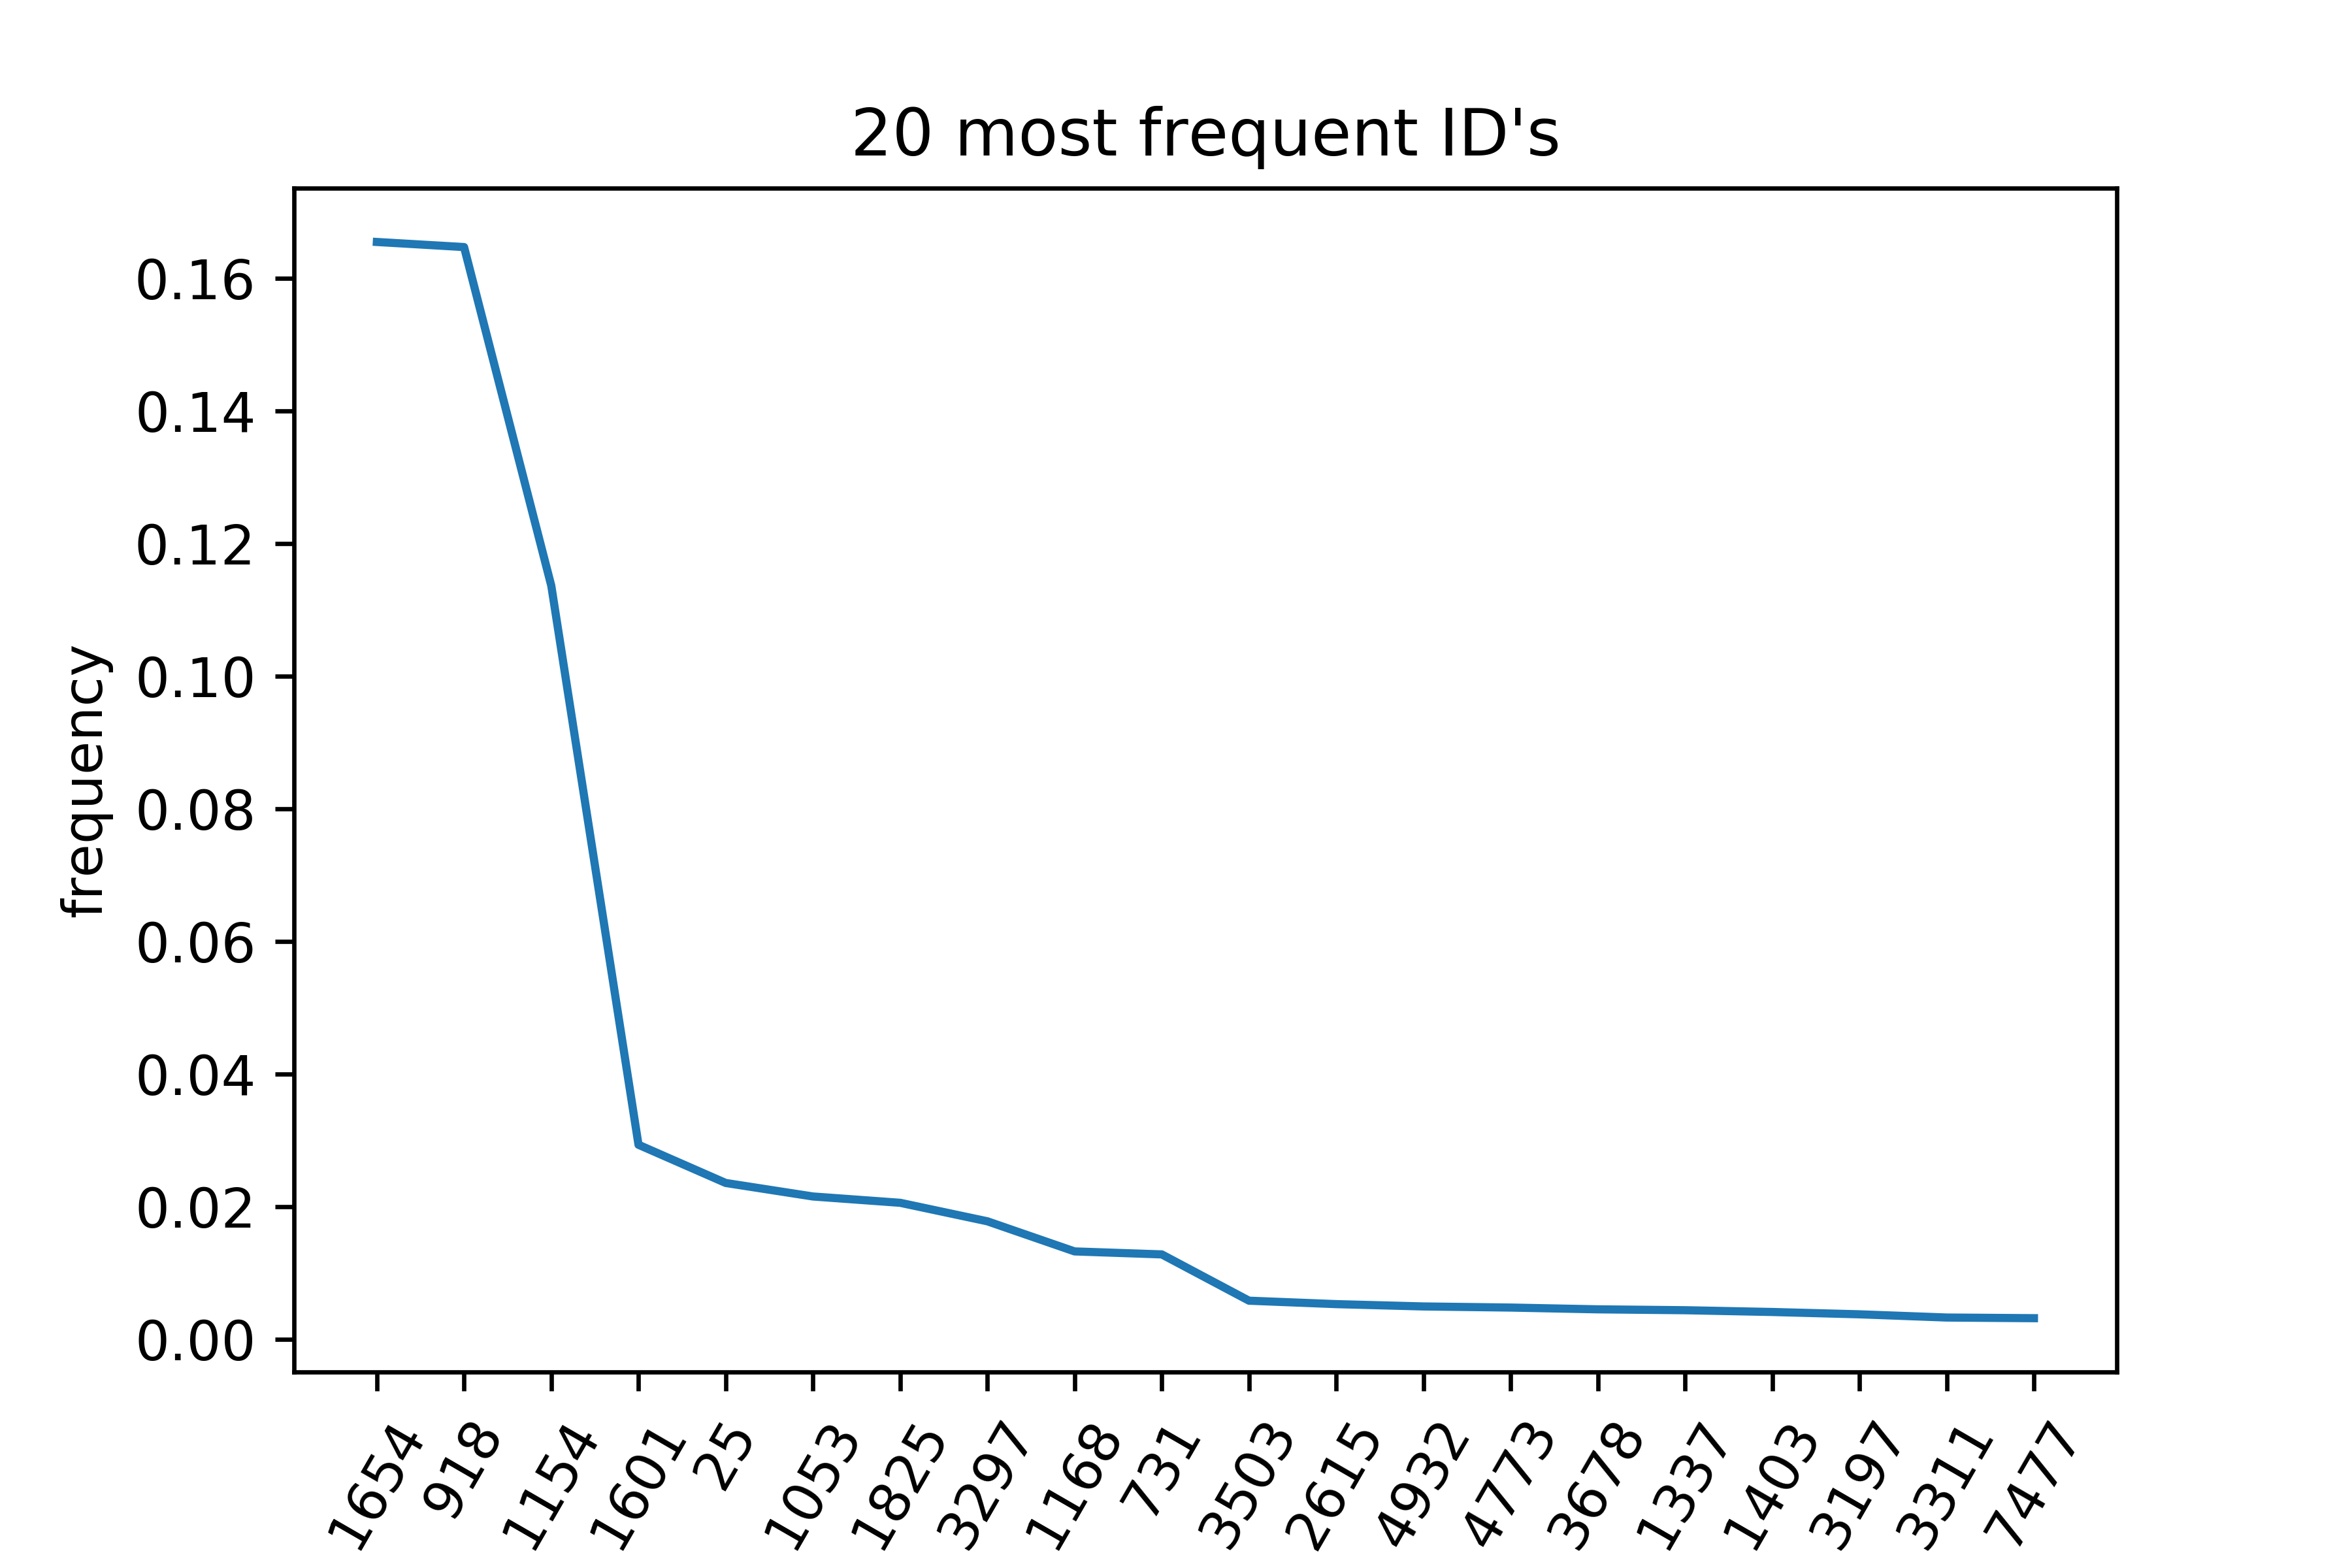
\includegraphics[scale=0.7]{figures/phylo1.png}
        \caption{\textbf{ID frequency} is shown for 20 most frequent ID's in the final population. The five most frequent IDs account for approx.\ $50\%$ of the population.}
        \label{fig1}
    \end{figure}

    \begin{figure}
        \center
        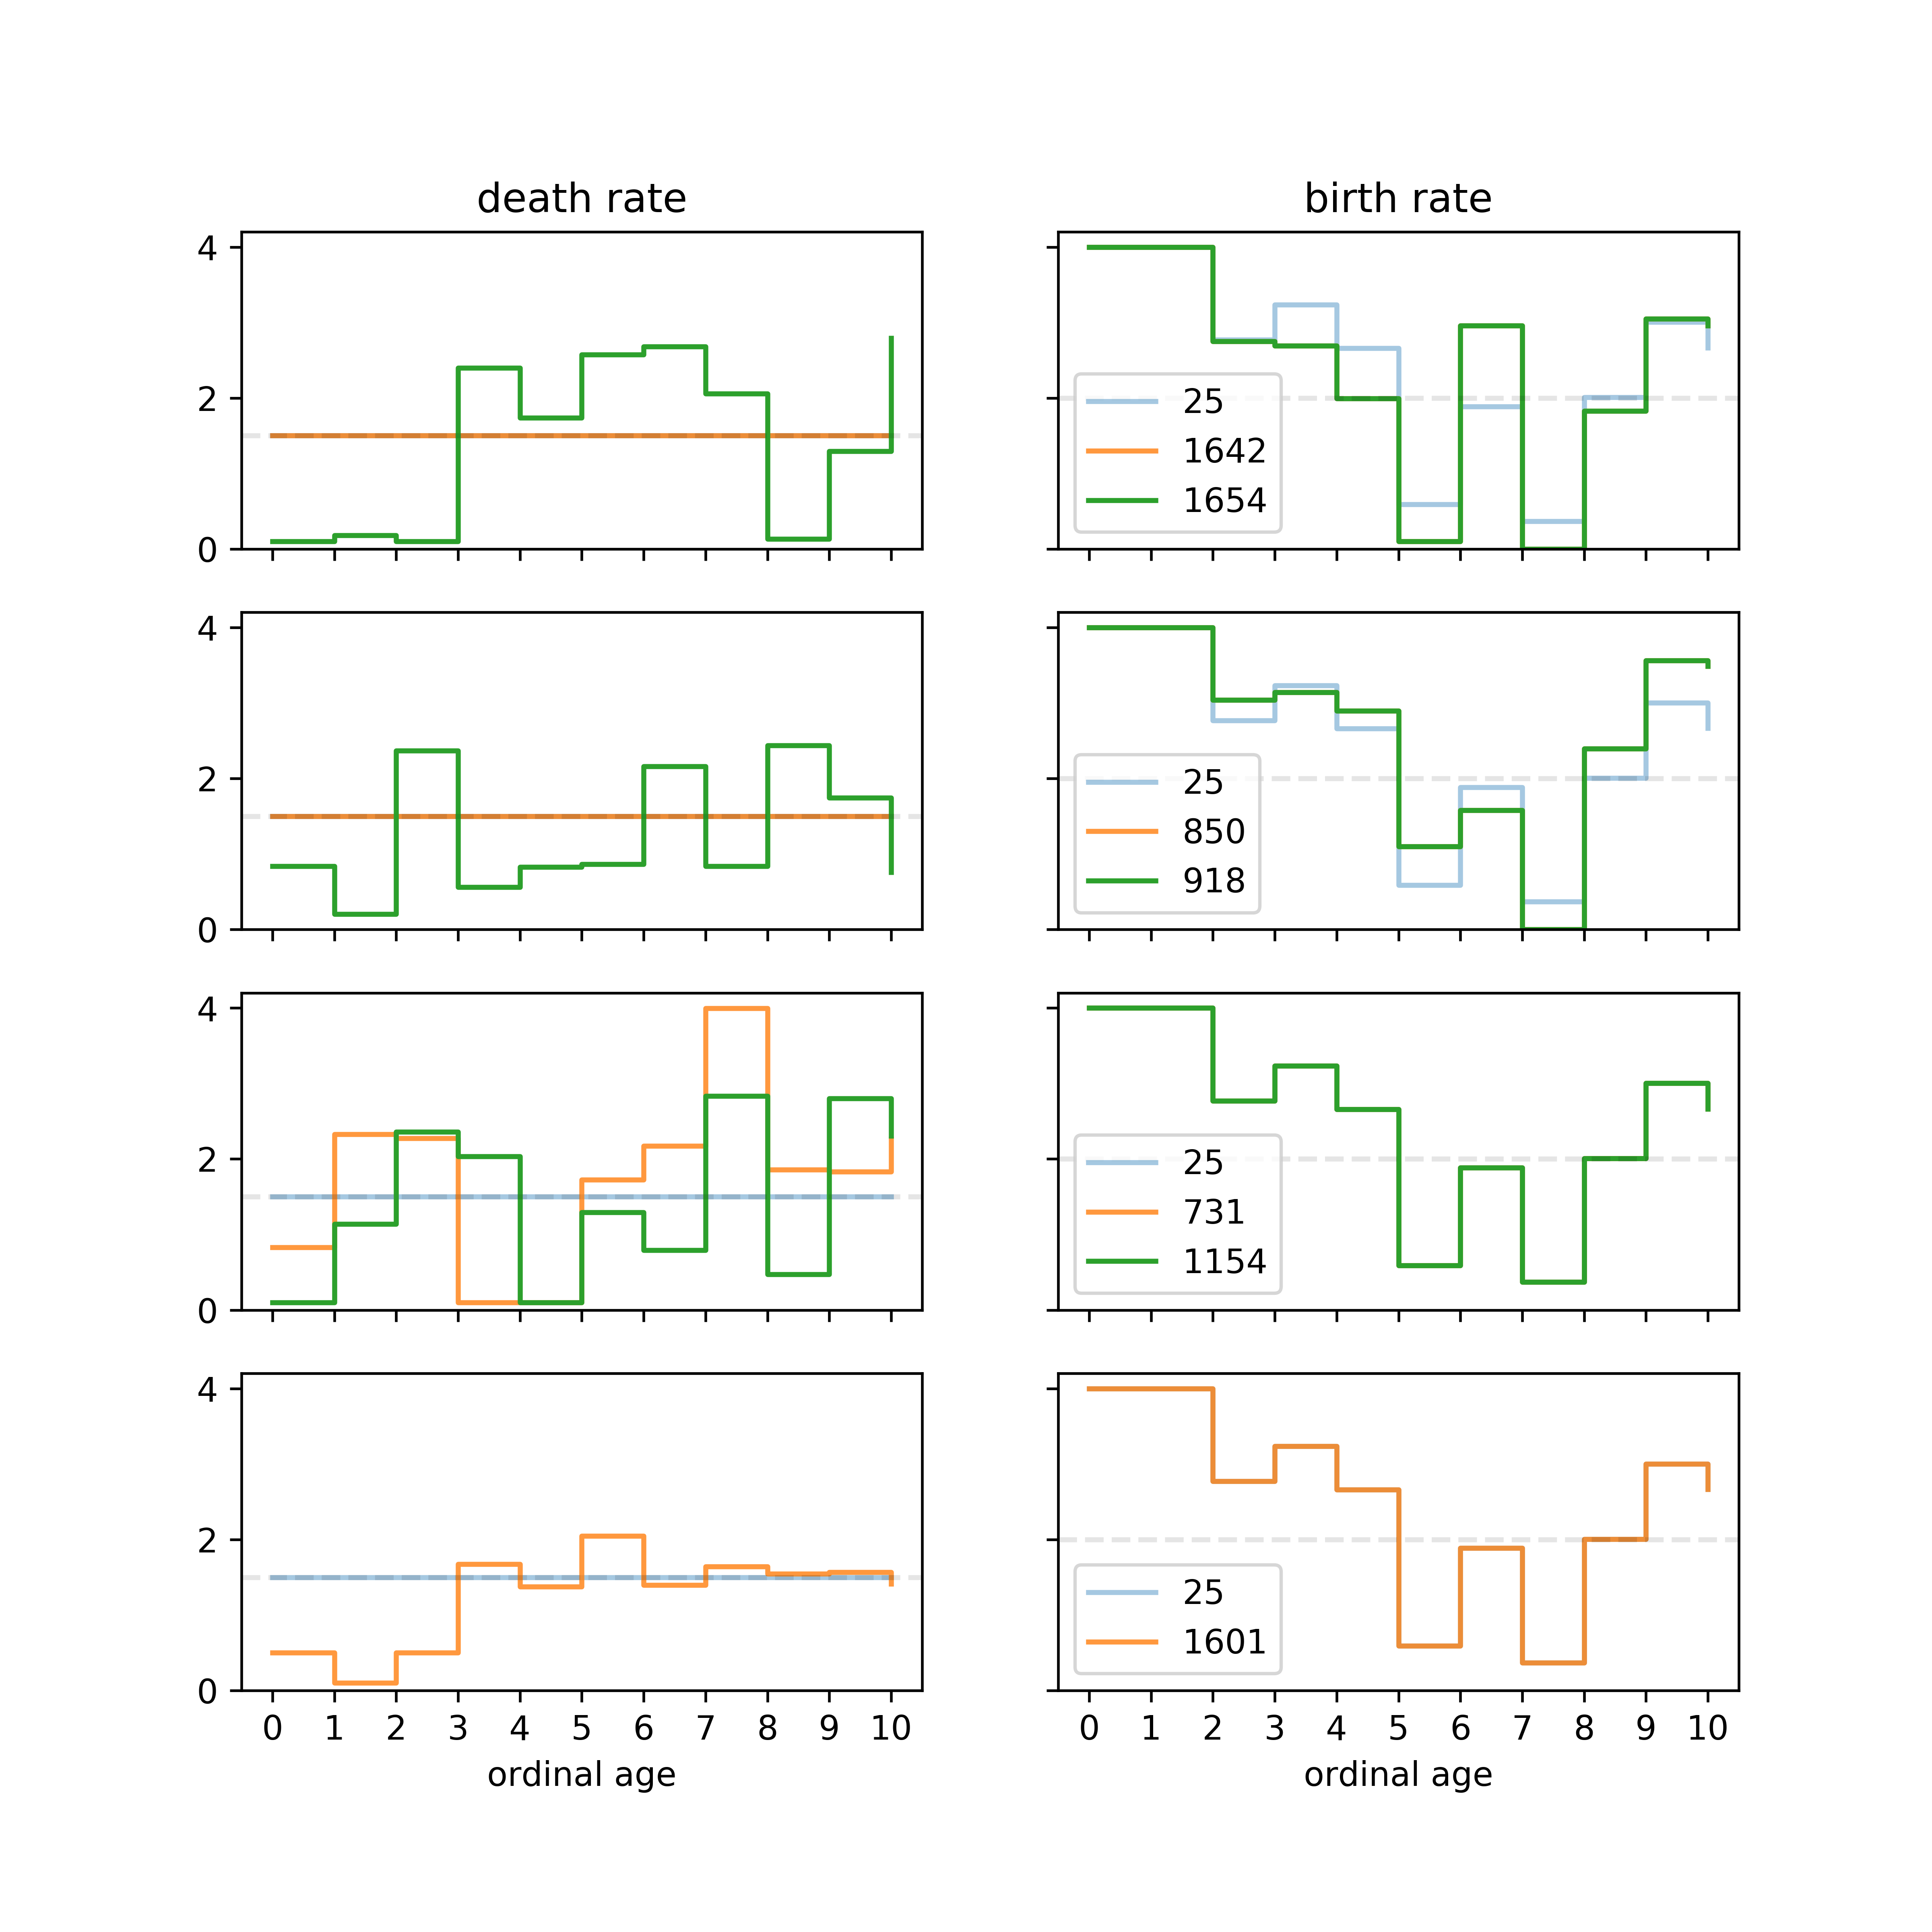
\includegraphics[width=\textwidth]{figures/phylo2.png}
        \caption{\textbf{Evolutionary history} of five most frequent IDs. Each column displays one trait: death or birth rate. Each row displays traits for one mutant lineage descended from ID $25$. On each axis, the dashed horizontal line marks the initial values of ID $0$, the pale blue line corresponds to ID $25$, the orange line corresponds to a child of ID $25$, and the green line corresponds to a grandchild of ID $25$. When no mutation has occurred for a trait from parent to child, the
        lines overlap and the child's line is drawn on top. Maximum age $a_{max}$ equals $2.0$.}
        \label{fig2}
    \end{figure}


\end{appendices}

\end{document}
